\begin{figure*}[h]
\centering
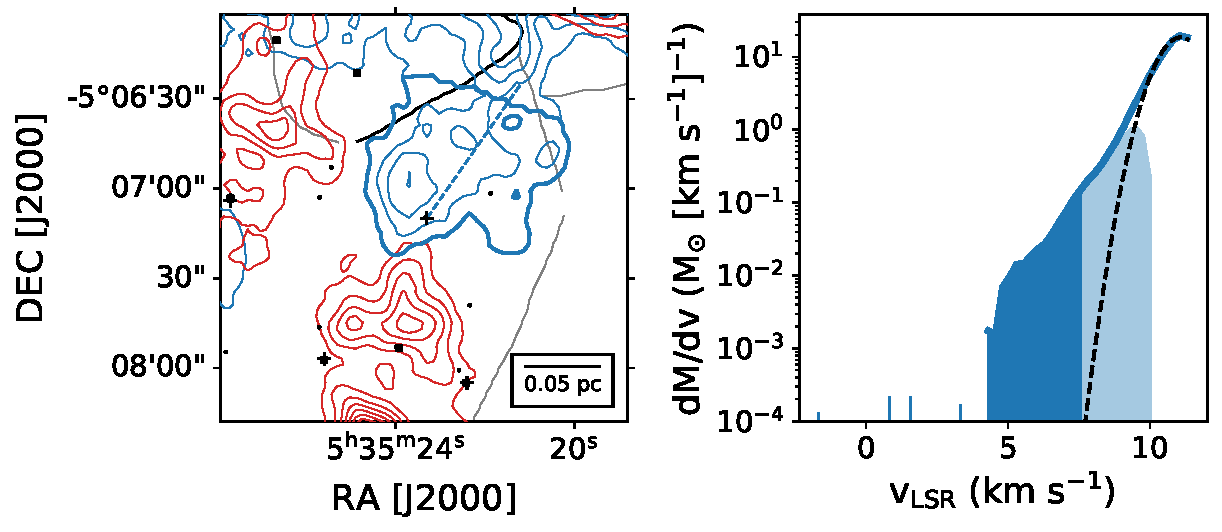
\includegraphics[width=\textwidth]{appendix_figures/davis11.pdf}

    \caption{SMZ 11 outflow. The left panel shows the outflow, position angle, nearby sources, and filaments.
    The velocity range of integration is given by v$_{\rm blue}$/v$_{\rm red}$ in Table~\ref{tab:outflows}
    and the contours go from $5$ to $50\sigma$ in steps of 5$\sigma$, where $\sigma$ is the RMS error in the integrated map. Symbols are the same as Figure~\ref{fig:stamp}.
    The right panel shows the mass spectrum with fit, where $\sigma$ is the RMS error in the integrated map. Symbols are the same as Figure~\ref{fig:dmdv}.}
    \end{figure*}
\begin{figure*}[h]
\centering
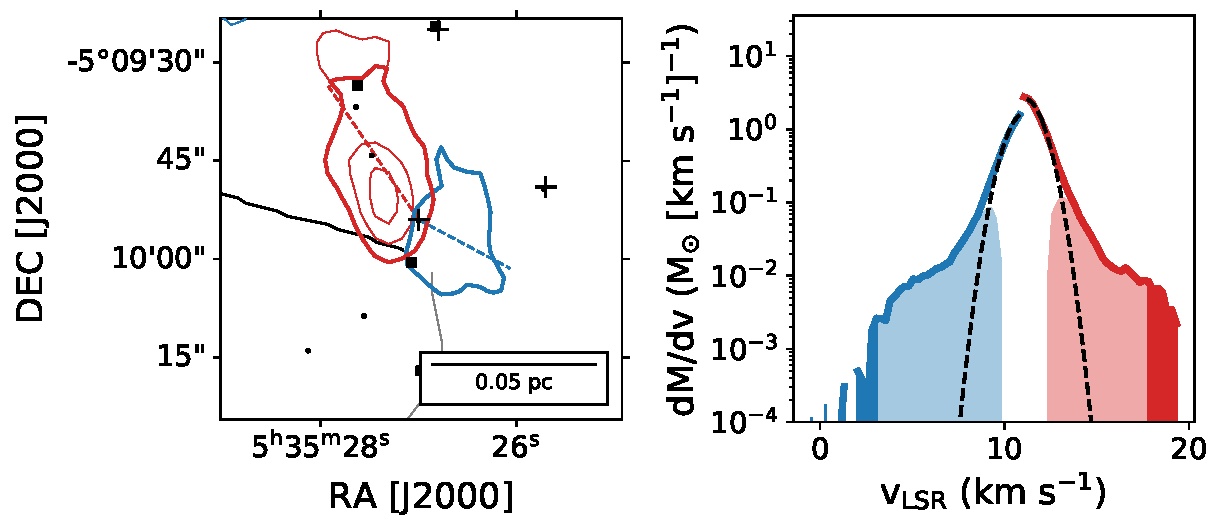
\includegraphics[width=\textwidth]{appendix_figures/davis17.pdf}

    \caption{SMZ 17 outflow. The left panel shows the outflow, position angle, nearby sources, and filaments.
    The velocity range of integration is given by v$_{\rm blue}$/v$_{\rm red}$ in Table~\ref{tab:outflows}
    and the contours go from $5$ to $50\sigma$ in steps of 5$\sigma$, where $\sigma$ is the RMS error in the integrated map. Symbols are the same as Figure~\ref{fig:stamp}.
    The right panel shows the mass spectrum with fit, where $\sigma$ is the RMS error in the integrated map. Symbols are the same as Figure~\ref{fig:dmdv}.}
    \end{figure*}
\begin{figure*}[p]
\centering
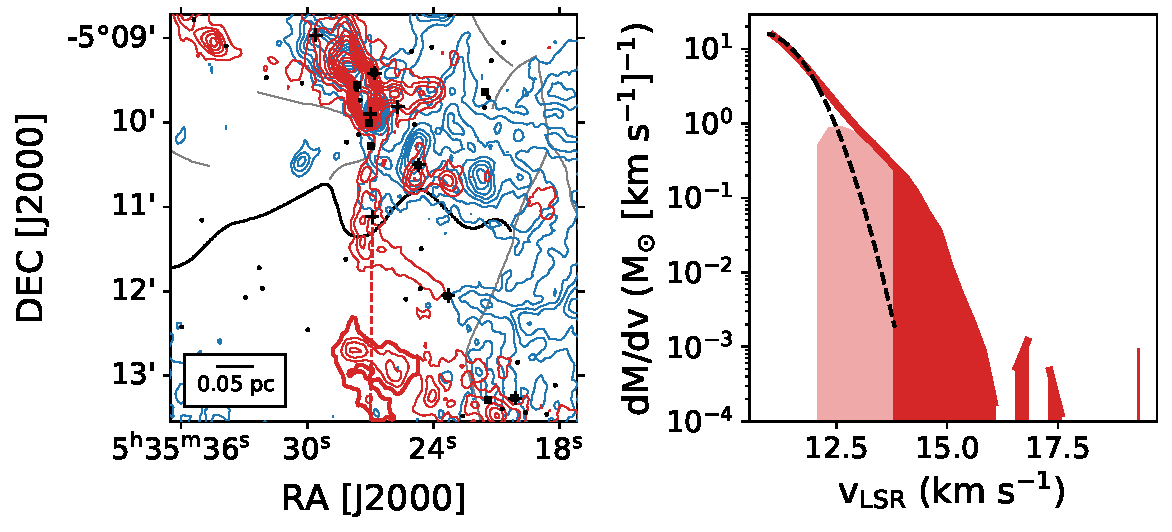
\includegraphics[width=\textwidth]{appendix_figures/davis21.pdf}

    \caption{SMZ 21 outflow. The left panel shows the outflow, position angle, nearby sources, and filaments.
    The velocity range of integration is given by v$_{\rm blue}$/v$_{\rm red}$ in Table~\ref{tab:outflows}
    and the contours go from $5$ to $50\sigma$ in steps of 5$\sigma$, where $\sigma$ is the RMS error in the integrated map. Symbols are the same as Figure~\ref{fig:stamp}.
    The right panel shows the mass spectrum with fit, where $\sigma$ is the RMS error in the integrated map. Symbols are the same as Figure~\ref{fig:dmdv}.}
    \end{figure*}
\begin{figure*}[p]
\centering
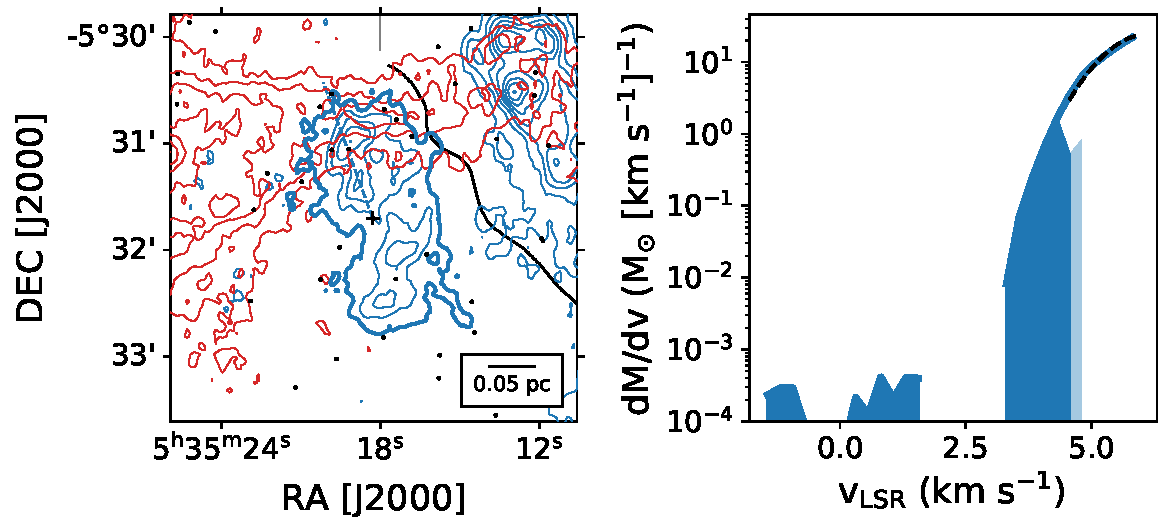
\includegraphics[width=\textwidth]{appendix_figures/davis30.pdf}

    \caption{SMZ 30 outflow. The left panel shows the outflow, position angle, nearby sources, and filaments.
    The velocity range of integration is given by v$_{\rm blue}$/v$_{\rm red}$ in Table~\ref{tab:outflows}
    and the contours go from $5$ to $50\sigma$ in steps of 5$\sigma$, where $\sigma$ is the RMS error in the integrated map. Symbols are the same as Figure~\ref{fig:stamp}.
    The right panel shows the mass spectrum with fit, where $\sigma$ is the RMS error in the integrated map. Symbols are the same as Figure~\ref{fig:dmdv}.}
    \end{figure*}
\begin{figure*}[p]
\centering
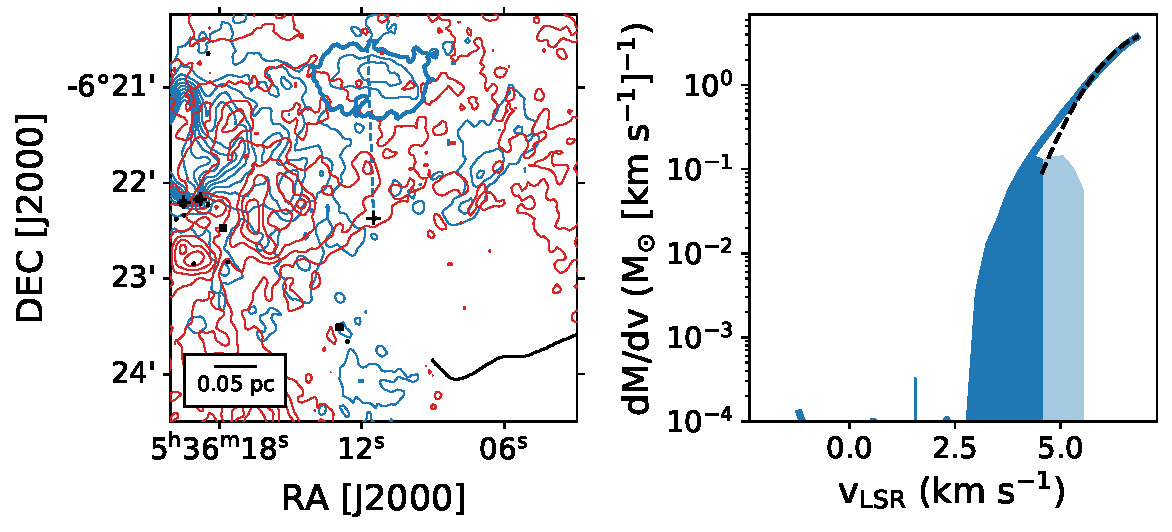
\includegraphics[width=\textwidth]{appendix_figures/davis50.pdf}

    \caption{SMZ 50 outflow. The left panel shows the outflow, position angle, nearby sources, and filaments.
    The velocity range of integration is given by v$_{\rm blue}$/v$_{\rm red}$ in Table~\ref{tab:outflows}
    and the contours go from $5$ to $50\sigma$ in steps of 5$\sigma$, where $\sigma$ is the RMS error in the integrated map. Symbols are the same as Figure~\ref{fig:stamp}.
    The right panel shows the mass spectrum with fit, where $\sigma$ is the RMS error in the integrated map. Symbols are the same as Figure~\ref{fig:dmdv}.}
    \end{figure*}
\begin{figure*}[p]
\centering
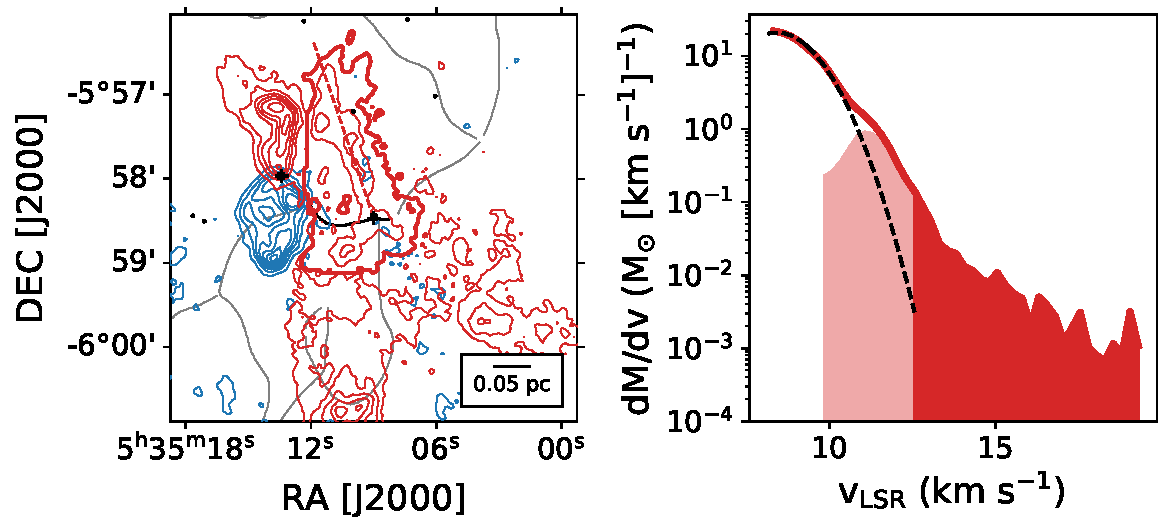
\includegraphics[width=\textwidth]{appendix_figures/hops10.pdf}

    \caption{HOPS 10 outflow. The left panel shows the outflow, position angle, nearby sources, and filaments.
    The velocity range of integration is given by v$_{\rm blue}$/v$_{\rm red}$ in Table~\ref{tab:outflows}
    and the contours go from $5$ to $50\sigma$ in steps of 5$\sigma$, where $\sigma$ is the RMS error in the integrated map. Symbols are the same as Figure~\ref{fig:stamp}.
    The right panel shows the mass spectrum with fit, where $\sigma$ is the RMS error in the integrated map. Symbols are the same as Figure~\ref{fig:dmdv}.}
    \end{figure*}
\begin{figure*}[p]
\centering
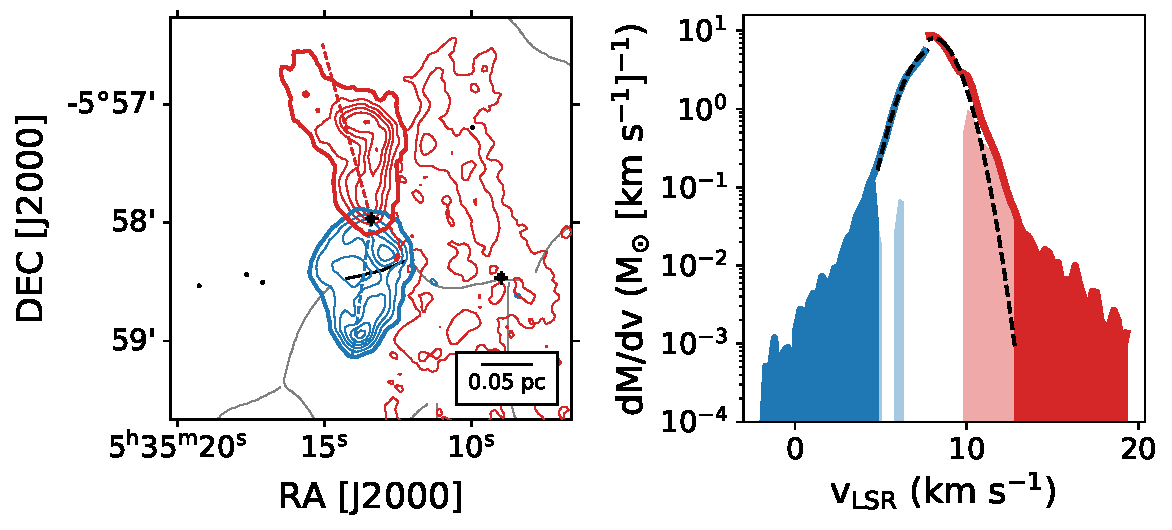
\includegraphics[width=\textwidth]{appendix_figures/hops11.pdf}

    \caption{HOPS 11 outflow. The left panel shows the outflow, position angle, nearby sources, and filaments.
    The velocity range of integration is given by v$_{\rm blue}$/v$_{\rm red}$ in Table~\ref{tab:outflows}
    and the contours go from $5$ to $50\sigma$ in steps of 5$\sigma$, where $\sigma$ is the RMS error in the integrated map. Symbols are the same as Figure~\ref{fig:stamp}.
    The right panel shows the mass spectrum with fit, where $\sigma$ is the RMS error in the integrated map. Symbols are the same as Figure~\ref{fig:dmdv}.}
    \end{figure*}
\begin{figure*}[p]
\centering
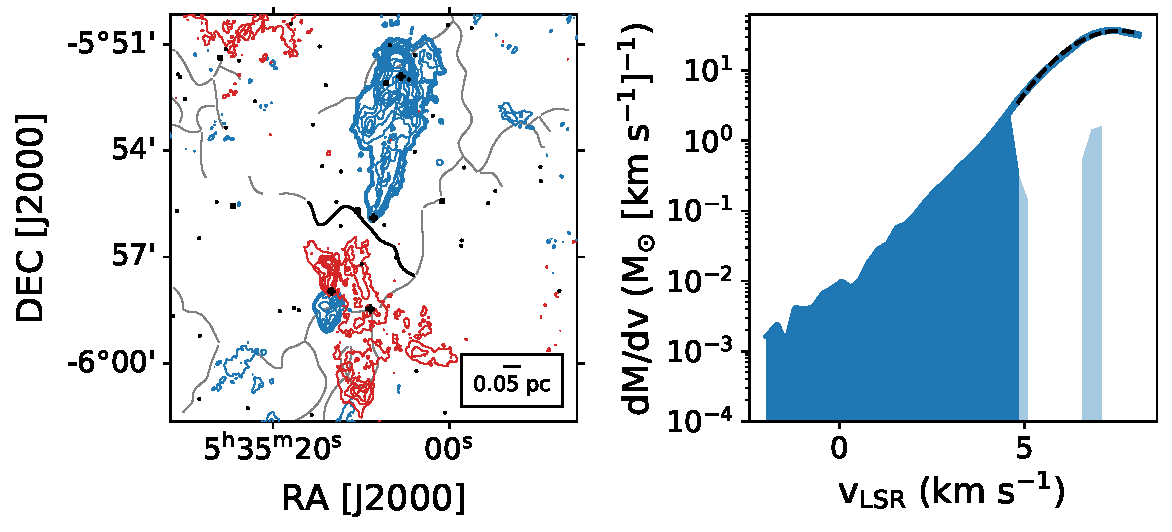
\includegraphics[width=\textwidth]{appendix_figures/hops12.pdf}

    \caption{HOPS 12 outflow. The left panel shows the outflow, position angle, nearby sources, and filaments.
    The velocity range of integration is given by v$_{\rm blue}$/v$_{\rm red}$ in Table~\ref{tab:outflows}
    and the contours go from $5$ to $50\sigma$ in steps of 5$\sigma$, where $\sigma$ is the RMS error in the integrated map. Symbols are the same as Figure~\ref{fig:stamp}.
    The right panel shows the mass spectrum with fit, where $\sigma$ is the RMS error in the integrated map. Symbols are the same as Figure~\ref{fig:dmdv}.}
    \end{figure*}
\begin{figure*}[p]
\centering
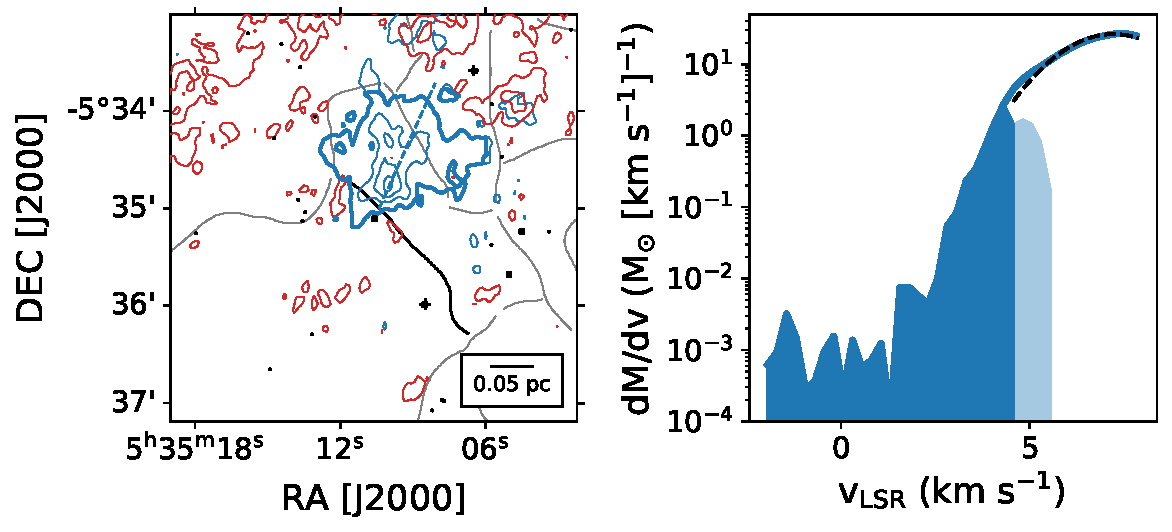
\includegraphics[width=\textwidth]{appendix_figures/hops44.pdf}

    \caption{HOPS 44 outflow. The left panel shows the outflow, position angle, nearby sources, and filaments.
    The velocity range of integration is given by v$_{\rm blue}$/v$_{\rm red}$ in Table~\ref{tab:outflows}
    and the contours go from $5$ to $50\sigma$ in steps of 5$\sigma$, where $\sigma$ is the RMS error in the integrated map. Symbols are the same as Figure~\ref{fig:stamp}.
    The right panel shows the mass spectrum with fit, where $\sigma$ is the RMS error in the integrated map. Symbols are the same as Figure~\ref{fig:dmdv}.}
    \end{figure*}
\begin{figure*}[p]
\centering
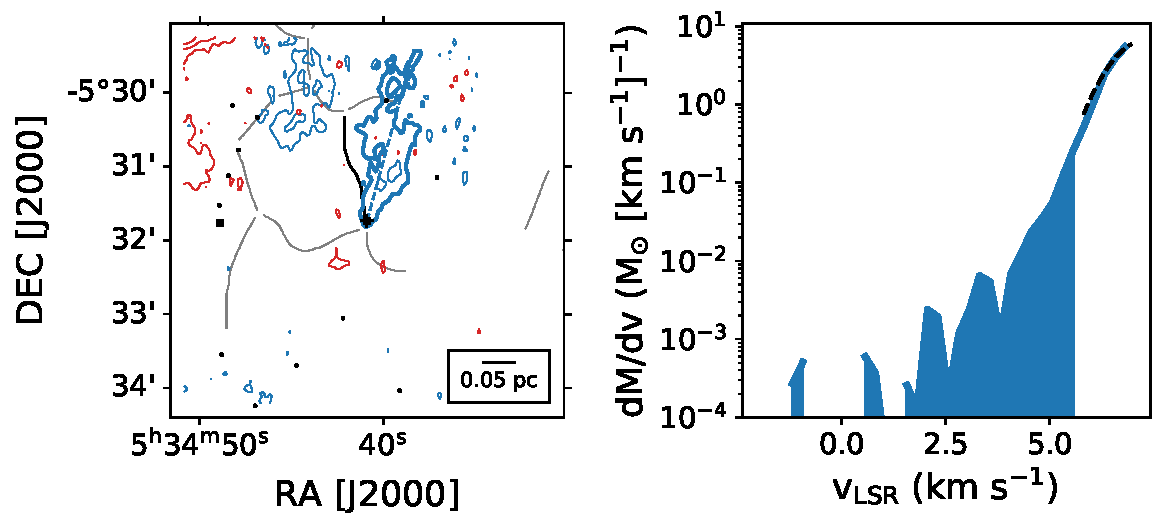
\includegraphics[width=\textwidth]{appendix_figures/hops50.pdf}

    \caption{HOPS 50 outflow. The left panel shows the outflow, position angle, nearby sources, and filaments.
    The velocity range of integration is given by v$_{\rm blue}$/v$_{\rm red}$ in Table~\ref{tab:outflows}
    and the contours go from $5$ to $50\sigma$ in steps of 5$\sigma$, where $\sigma$ is the RMS error in the integrated map. Symbols are the same as Figure~\ref{fig:stamp}.
    The right panel shows the mass spectrum with fit, where $\sigma$ is the RMS error in the integrated map. Symbols are the same as Figure~\ref{fig:dmdv}.}
    \end{figure*}
\begin{figure*}[p]
\centering
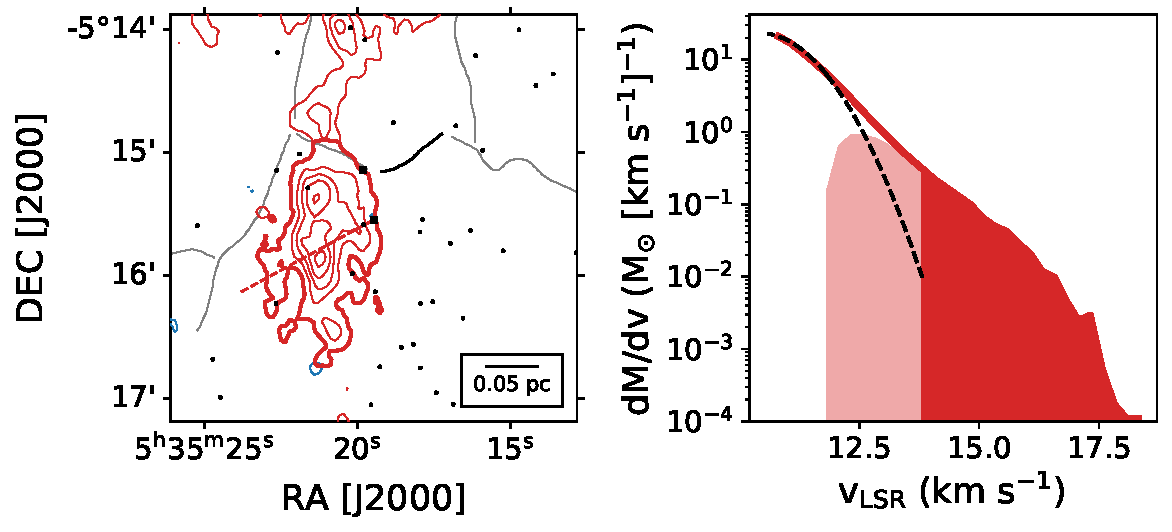
\includegraphics[width=\textwidth]{appendix_figures/hops56.pdf}

    \caption{HOPS 56 outflow. The left panel shows the outflow, position angle, nearby sources, and filaments.
    The velocity range of integration is given by v$_{\rm blue}$/v$_{\rm red}$ in Table~\ref{tab:outflows}
    and the contours go from $5$ to $50\sigma$ in steps of 5$\sigma$, where $\sigma$ is the RMS error in the integrated map. Symbols are the same as Figure~\ref{fig:stamp}.
    The right panel shows the mass spectrum with fit, where $\sigma$ is the RMS error in the integrated map. Symbols are the same as Figure~\ref{fig:dmdv}.}
    \end{figure*}
\begin{figure*}[p]
\centering
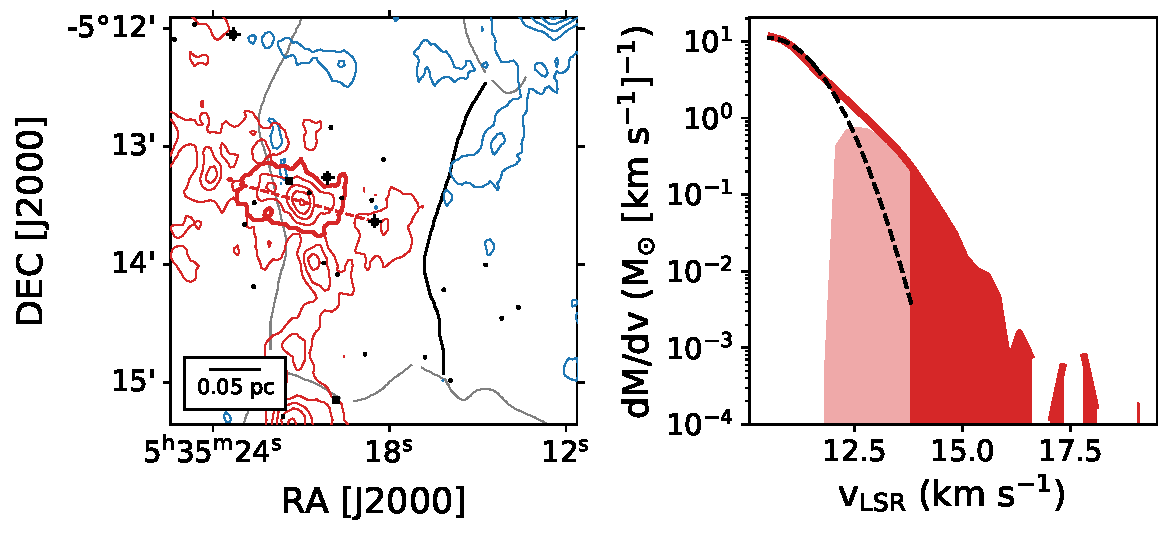
\includegraphics[width=\textwidth]{appendix_figures/hops58.pdf}

    \caption{HOPS 58 outflow. The left panel shows the outflow, position angle, nearby sources, and filaments.
    The velocity range of integration is given by v$_{\rm blue}$/v$_{\rm red}$ in Table~\ref{tab:outflows}
    and the contours go from $5$ to $50\sigma$ in steps of 5$\sigma$, where $\sigma$ is the RMS error in the integrated map. Symbols are the same as Figure~\ref{fig:stamp}.
    The right panel shows the mass spectrum with fit, where $\sigma$ is the RMS error in the integrated map. Symbols are the same as Figure~\ref{fig:dmdv}.}
    \end{figure*}
\begin{figure*}[p]
\centering
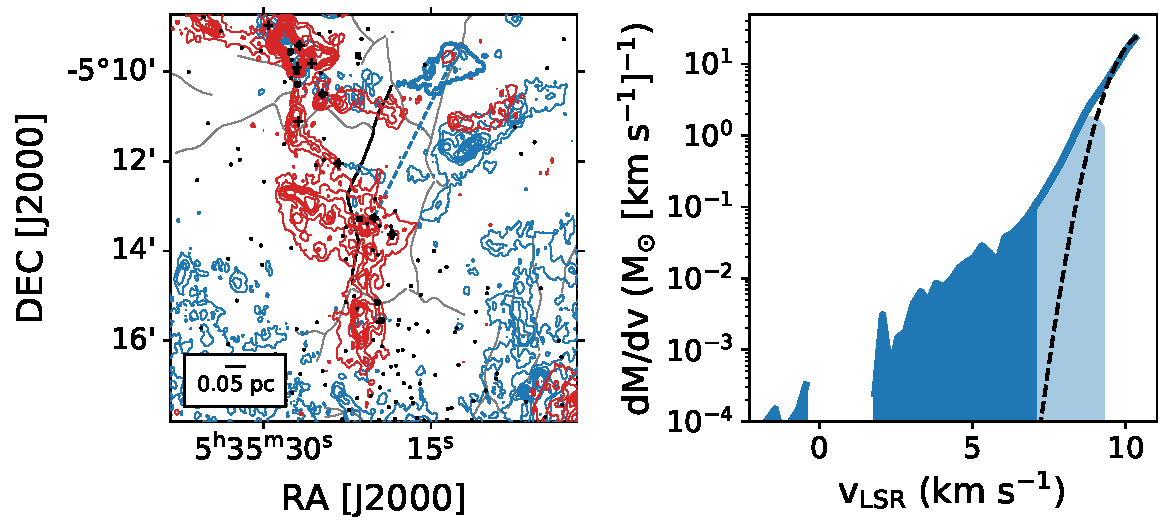
\includegraphics[width=\textwidth]{appendix_figures/hops59.pdf}

    \caption{HOPS 59 outflow. The left panel shows the outflow, position angle, nearby sources, and filaments.
    The velocity range of integration is given by v$_{\rm blue}$/v$_{\rm red}$ in Table~\ref{tab:outflows}
    and the contours go from $5$ to $50\sigma$ in steps of 5$\sigma$, where $\sigma$ is the RMS error in the integrated map. Symbols are the same as Figure~\ref{fig:stamp}.
    The right panel shows the mass spectrum with fit, where $\sigma$ is the RMS error in the integrated map. Symbols are the same as Figure~\ref{fig:dmdv}.}
    \end{figure*}
\begin{figure*}[p]
\centering
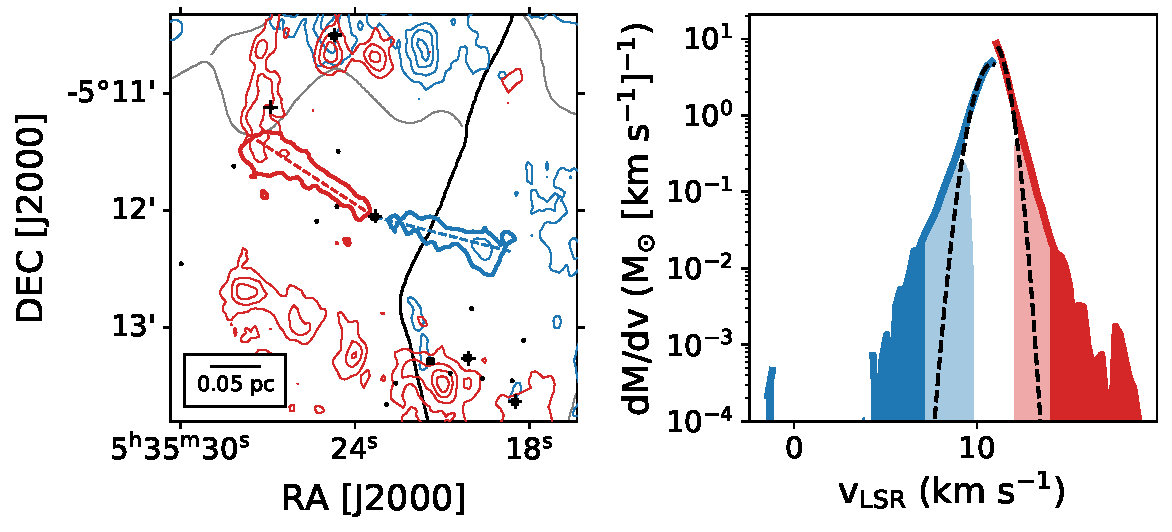
\includegraphics[width=\textwidth]{appendix_figures/hops60.pdf}

    \caption{HOPS 60 outflow. The left panel shows the outflow, position angle, nearby sources, and filaments.
    The velocity range of integration is given by v$_{\rm blue}$/v$_{\rm red}$ in Table~\ref{tab:outflows}
    and the contours go from $5$ to $50\sigma$ in steps of 5$\sigma$, where $\sigma$ is the RMS error in the integrated map. Symbols are the same as Figure~\ref{fig:stamp}.
    The right panel shows the mass spectrum with fit, where $\sigma$ is the RMS error in the integrated map. Symbols are the same as Figure~\ref{fig:dmdv}.}
    \end{figure*}
\begin{figure*}[p]
\centering
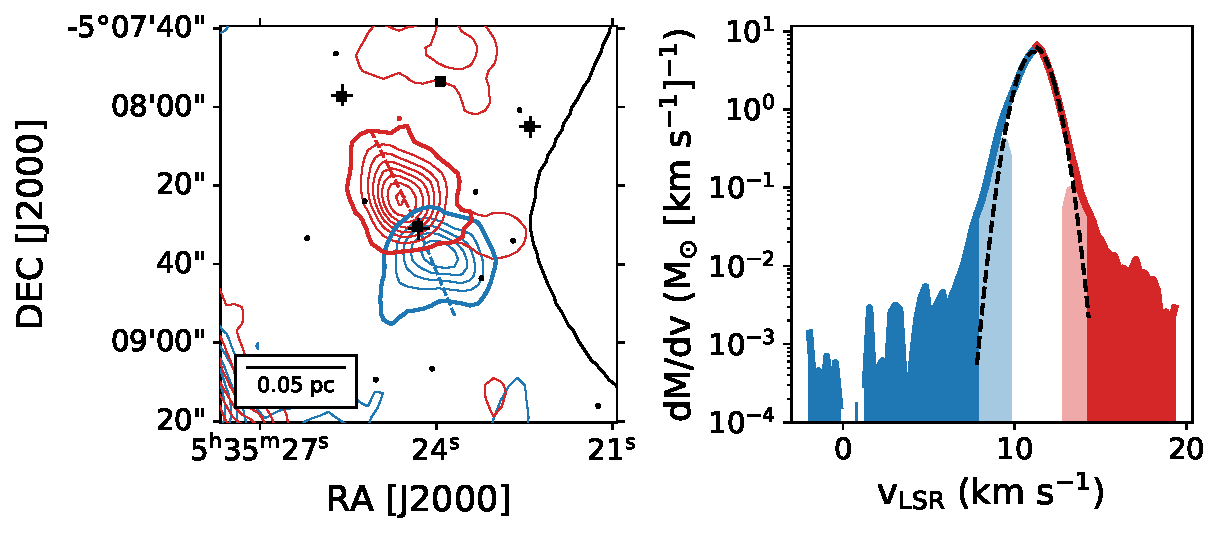
\includegraphics[width=\textwidth]{appendix_figures/hops68.pdf}

    \caption{HOPS 68 outflow. The left panel shows the outflow, position angle, nearby sources, and filaments.
    The velocity range of integration is given by v$_{\rm blue}$/v$_{\rm red}$ in Table~\ref{tab:outflows}
    and the contours go from $5$ to $50\sigma$ in steps of 5$\sigma$, where $\sigma$ is the RMS error in the integrated map. Symbols are the same as Figure~\ref{fig:stamp}.
    The right panel shows the mass spectrum with fit, where $\sigma$ is the RMS error in the integrated map. Symbols are the same as Figure~\ref{fig:dmdv}.}
    \end{figure*}
\begin{figure*}[p]
\centering
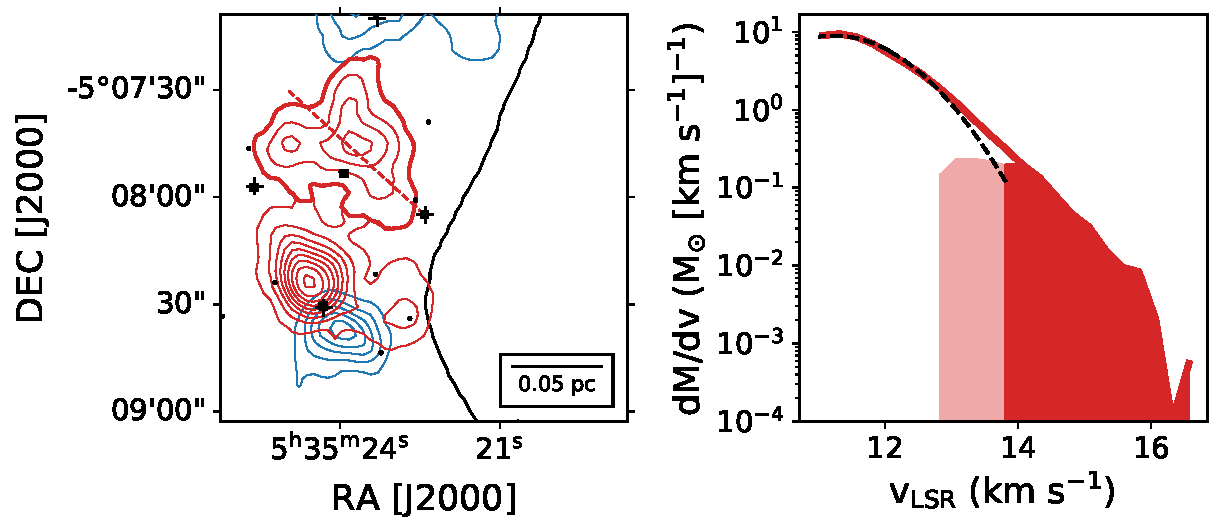
\includegraphics[width=\textwidth]{appendix_figures/hops70.pdf}

    \caption{HOPS 70 outflow. The left panel shows the outflow, position angle, nearby sources, and filaments.
    The velocity range of integration is given by v$_{\rm blue}$/v$_{\rm red}$ in Table~\ref{tab:outflows}
    and the contours go from $5$ to $50\sigma$ in steps of 5$\sigma$, where $\sigma$ is the RMS error in the integrated map. Symbols are the same as Figure~\ref{fig:stamp}.
    The right panel shows the mass spectrum with fit, where $\sigma$ is the RMS error in the integrated map. Symbols are the same as Figure~\ref{fig:dmdv}.}
    \end{figure*}
\begin{figure*}[p]
\centering
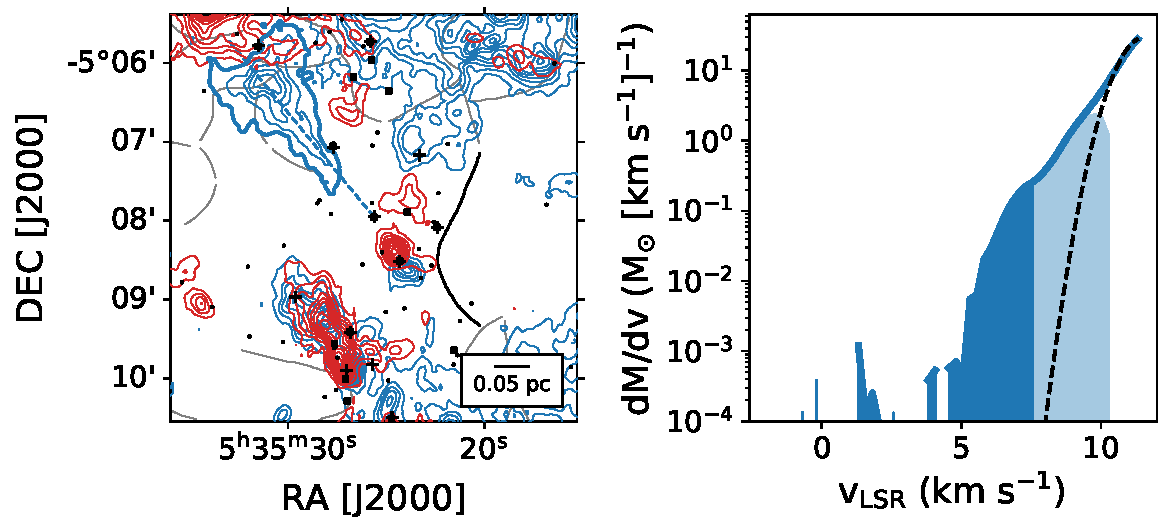
\includegraphics[width=\textwidth]{appendix_figures/hops71.pdf}

    \caption{HOPS 71 outflow. The left panel shows the outflow, position angle, nearby sources, and filaments.
    The velocity range of integration is given by v$_{\rm blue}$/v$_{\rm red}$ in Table~\ref{tab:outflows}
    and the contours go from $5$ to $50\sigma$ in steps of 5$\sigma$, where $\sigma$ is the RMS error in the integrated map. Symbols are the same as Figure~\ref{fig:stamp}.
    The right panel shows the mass spectrum with fit, where $\sigma$ is the RMS error in the integrated map. Symbols are the same as Figure~\ref{fig:dmdv}.}
    \end{figure*}
\begin{figure*}[p]
\centering
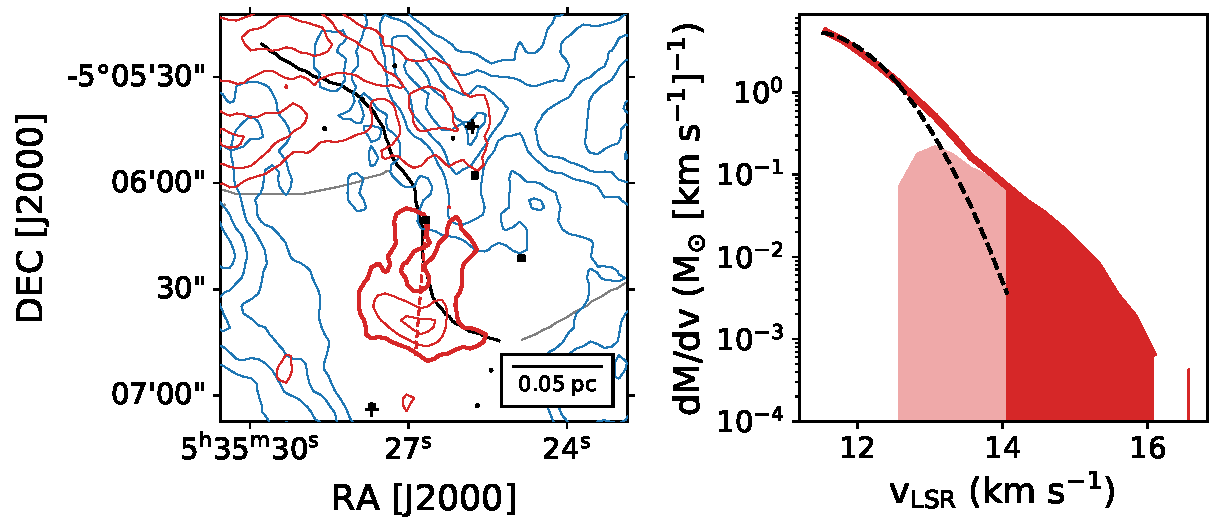
\includegraphics[width=\textwidth]{appendix_figures/hops75.pdf}

    \caption{HOPS 75 outflow. The left panel shows the outflow, position angle, nearby sources, and filaments.
    The velocity range of integration is given by v$_{\rm blue}$/v$_{\rm red}$ in Table~\ref{tab:outflows}
    and the contours go from $5$ to $50\sigma$ in steps of 5$\sigma$, where $\sigma$ is the RMS error in the integrated map. Symbols are the same as Figure~\ref{fig:stamp}.
    The right panel shows the mass spectrum with fit, where $\sigma$ is the RMS error in the integrated map. Symbols are the same as Figure~\ref{fig:dmdv}.}
    \end{figure*}
\begin{figure*}[p]
\centering
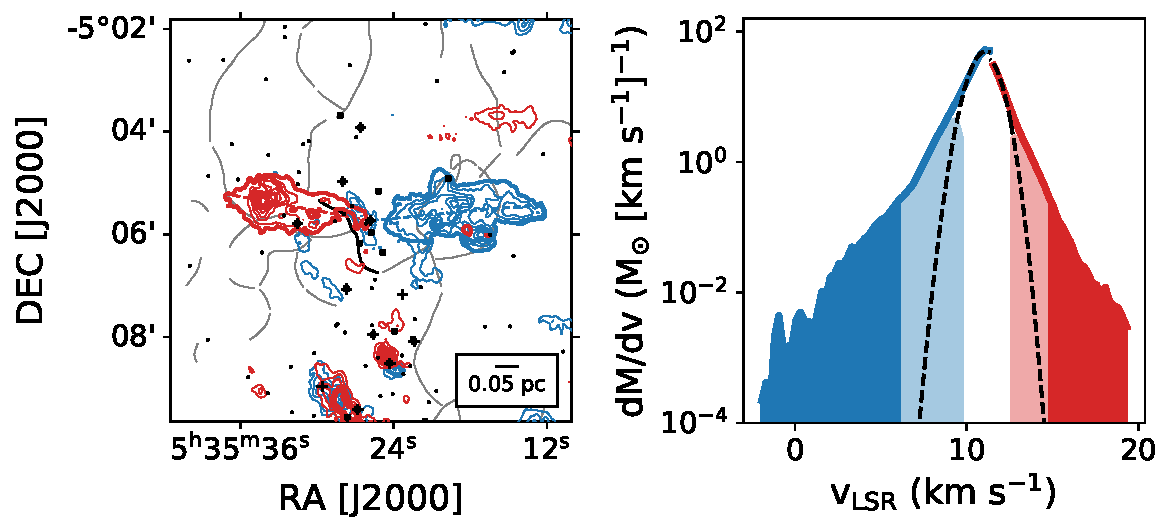
\includegraphics[width=\textwidth]{appendix_figures/hops78.pdf}

    \caption{HOPS 78 outflow. The left panel shows the outflow, position angle, nearby sources, and filaments.
    The velocity range of integration is given by v$_{\rm blue}$/v$_{\rm red}$ in Table~\ref{tab:outflows}
    and the contours go from $5$ to $50\sigma$ in steps of 5$\sigma$, where $\sigma$ is the RMS error in the integrated map. Symbols are the same as Figure~\ref{fig:stamp}.
    The right panel shows the mass spectrum with fit, where $\sigma$ is the RMS error in the integrated map. Symbols are the same as Figure~\ref{fig:dmdv}.}
    \end{figure*}
\begin{figure*}[p]
\centering
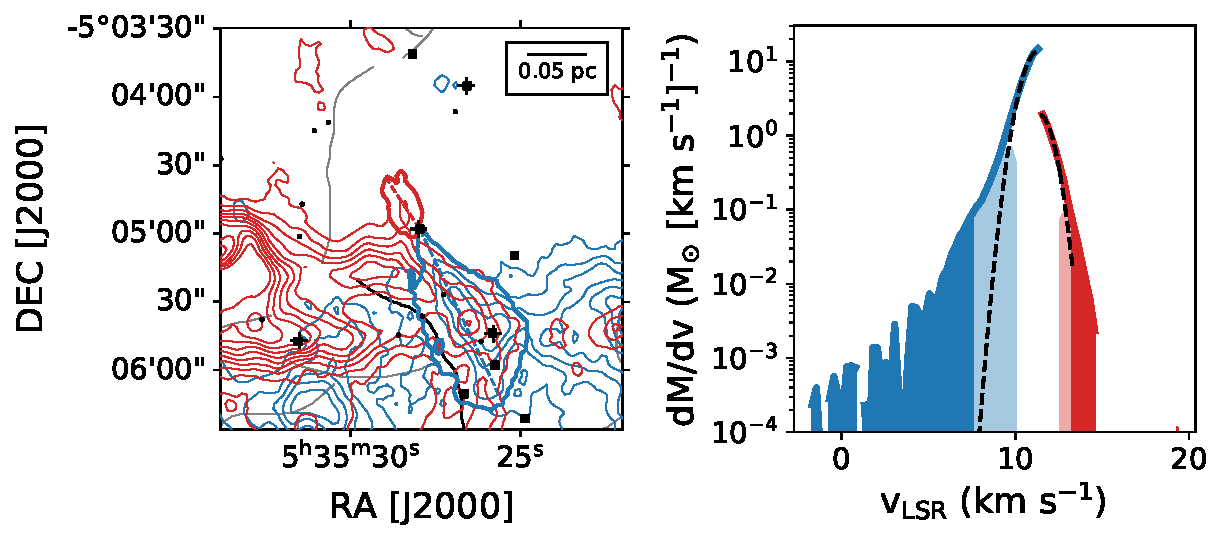
\includegraphics[width=\textwidth]{appendix_figures/hops81.pdf}

    \caption{HOPS 81 outflow. The left panel shows the outflow, position angle, nearby sources, and filaments.
    The velocity range of integration is given by v$_{\rm blue}$/v$_{\rm red}$ in Table~\ref{tab:outflows}
    and the contours go from $5$ to $50\sigma$ in steps of 5$\sigma$, where $\sigma$ is the RMS error in the integrated map. Symbols are the same as Figure~\ref{fig:stamp}.
    The right panel shows the mass spectrum with fit, where $\sigma$ is the RMS error in the integrated map. Symbols are the same as Figure~\ref{fig:dmdv}.}
    \end{figure*}
\begin{figure*}[p]
\centering
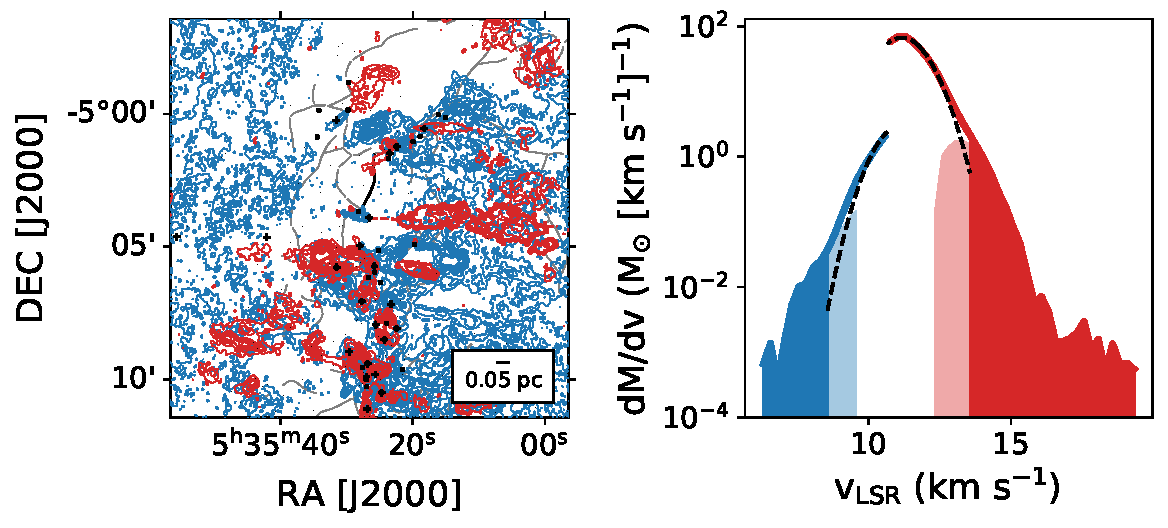
\includegraphics[width=\textwidth]{appendix_figures/hops84.pdf}

    \caption{HOPS 84 outflow. The left panel shows the outflow, position angle, nearby sources, and filaments.
    The velocity range of integration is given by v$_{\rm blue}$/v$_{\rm red}$ in Table~\ref{tab:outflows}
    and the contours go from $5$ to $50\sigma$ in steps of 5$\sigma$, where $\sigma$ is the RMS error in the integrated map. Symbols are the same as Figure~\ref{fig:stamp}.
    The right panel shows the mass spectrum with fit, where $\sigma$ is the RMS error in the integrated map. Symbols are the same as Figure~\ref{fig:dmdv}.}
    \end{figure*}
\begin{figure*}[p]
\centering
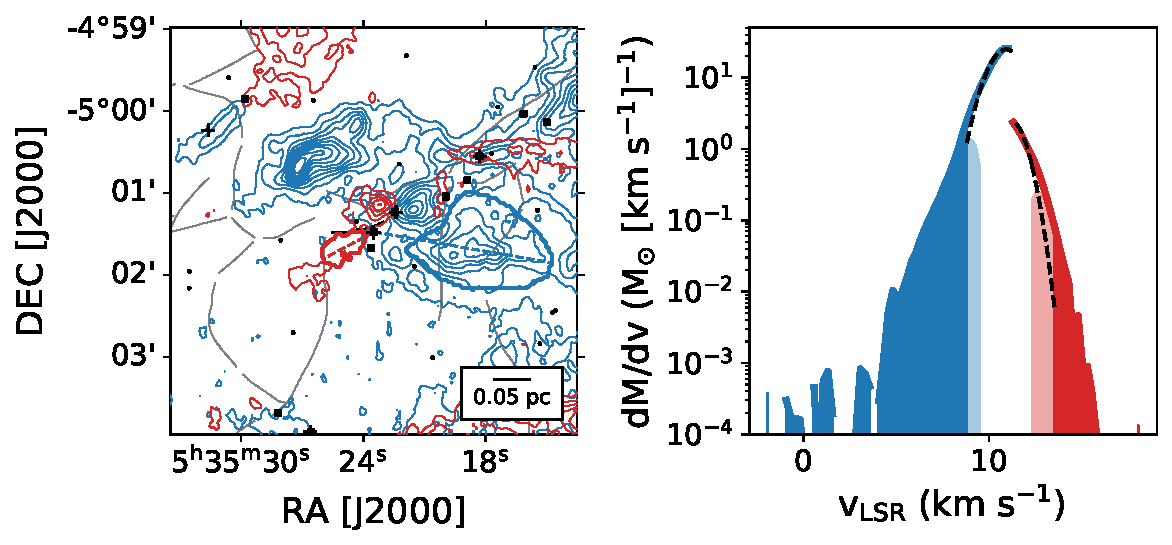
\includegraphics[width=\textwidth]{appendix_figures/hops87.pdf}

    \caption{HOPS 87 outflow. The left panel shows the outflow, position angle, nearby sources, and filaments.
    The velocity range of integration is given by v$_{\rm blue}$/v$_{\rm red}$ in Table~\ref{tab:outflows}
    and the contours go from $5$ to $50\sigma$ in steps of 5$\sigma$, where $\sigma$ is the RMS error in the integrated map. Symbols are the same as Figure~\ref{fig:stamp}.
    The right panel shows the mass spectrum with fit, where $\sigma$ is the RMS error in the integrated map. Symbols are the same as Figure~\ref{fig:dmdv}.}
    \end{figure*}
\begin{figure*}[p]
\centering
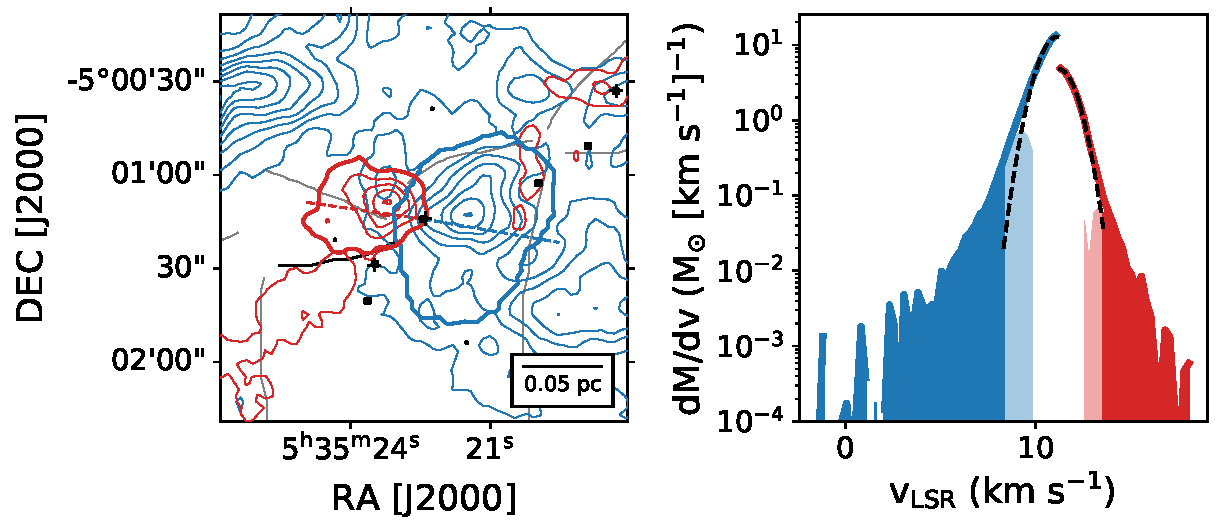
\includegraphics[width=\textwidth]{appendix_figures/hops88.pdf}

    \caption{HOPS 88 outflow. The left panel shows the outflow, position angle, nearby sources, and filaments.
    The velocity range of integration is given by v$_{\rm blue}$/v$_{\rm red}$ in Table~\ref{tab:outflows}
    and the contours go from $5$ to $50\sigma$ in steps of 5$\sigma$, where $\sigma$ is the RMS error in the integrated map. Symbols are the same as Figure~\ref{fig:stamp}.
    The right panel shows the mass spectrum with fit, where $\sigma$ is the RMS error in the integrated map. Symbols are the same as Figure~\ref{fig:dmdv}.}
    \end{figure*}
\begin{figure*}[p]
\centering
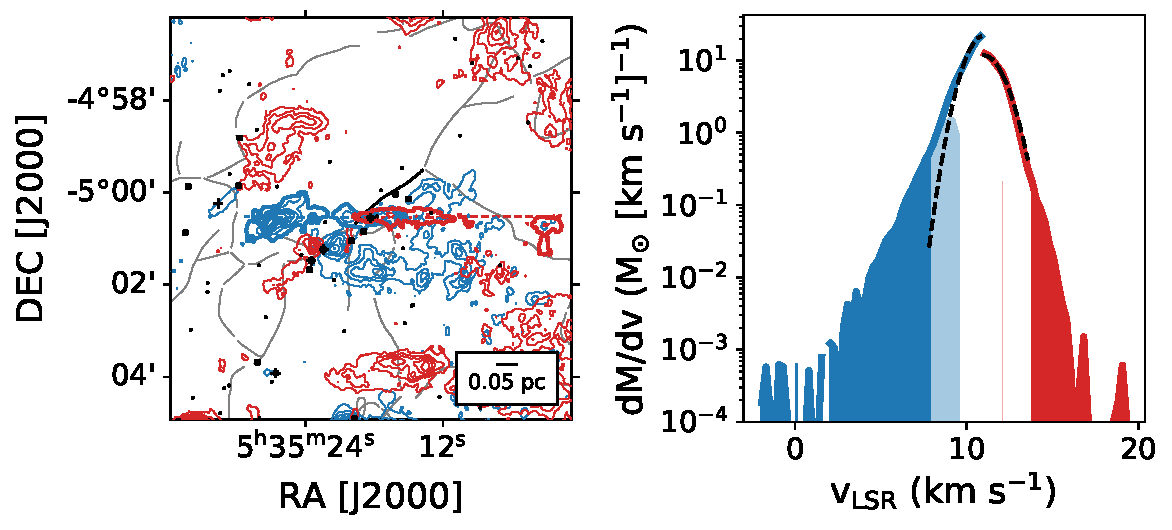
\includegraphics[width=\textwidth]{appendix_figures/hops92.pdf}

    \caption{HOPS 92 outflow. The left panel shows the outflow, position angle, nearby sources, and filaments.
    The velocity range of integration is given by v$_{\rm blue}$/v$_{\rm red}$ in Table~\ref{tab:outflows}
    and the contours go from $5$ to $50\sigma$ in steps of 5$\sigma$, where $\sigma$ is the RMS error in the integrated map. Symbols are the same as Figure~\ref{fig:stamp}.
    The right panel shows the mass spectrum with fit, where $\sigma$ is the RMS error in the integrated map. Symbols are the same as Figure~\ref{fig:dmdv}.}
    \end{figure*}
\begin{figure*}[p]
\centering
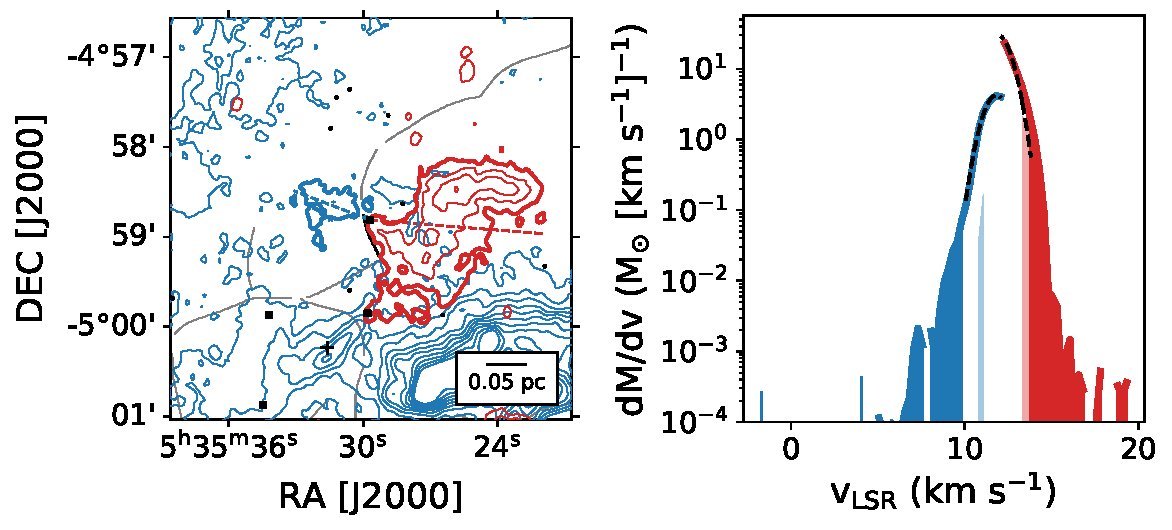
\includegraphics[width=\textwidth]{appendix_figures/hops96.pdf}

    \caption{HOPS 96 outflow. The left panel shows the outflow, position angle, nearby sources, and filaments.
    The velocity range of integration is given by v$_{\rm blue}$/v$_{\rm red}$ in Table~\ref{tab:outflows}
    and the contours go from $5$ to $50\sigma$ in steps of 5$\sigma$, where $\sigma$ is the RMS error in the integrated map. Symbols are the same as Figure~\ref{fig:stamp}.
    The right panel shows the mass spectrum with fit, where $\sigma$ is the RMS error in the integrated map. Symbols are the same as Figure~\ref{fig:dmdv}.}
    \end{figure*}
\begin{figure*}[p]
\centering
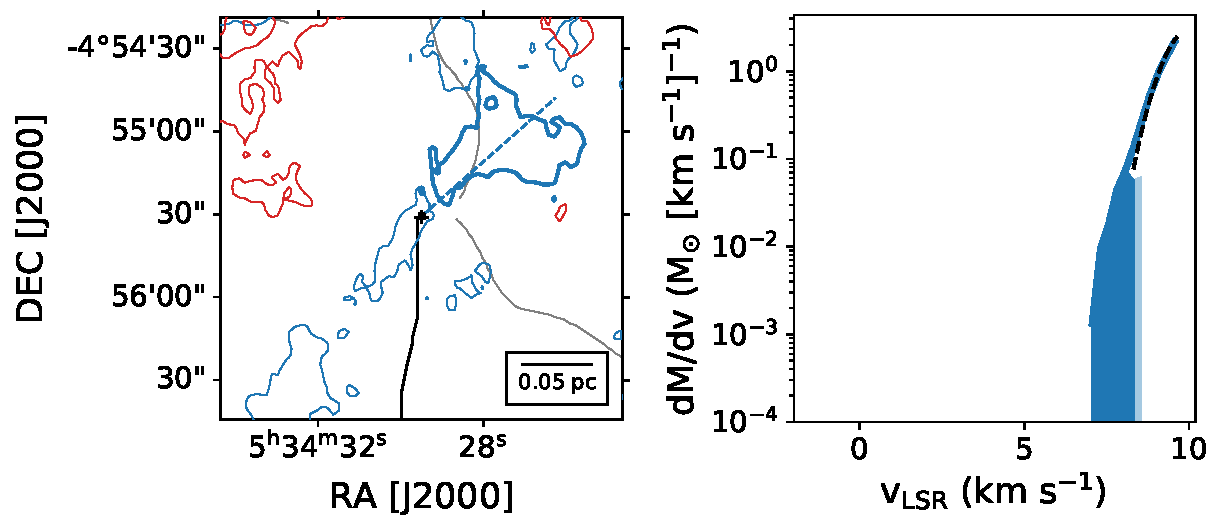
\includegraphics[width=\textwidth]{appendix_figures/hops99.pdf}

    \caption{HOPS 99 outflow. The left panel shows the outflow, position angle, nearby sources, and filaments.
    The velocity range of integration is given by v$_{\rm blue}$/v$_{\rm red}$ in Table~\ref{tab:outflows}
    and the contours go from $5$ to $50\sigma$ in steps of 5$\sigma$, where $\sigma$ is the RMS error in the integrated map. Symbols are the same as Figure~\ref{fig:stamp}.
    The right panel shows the mass spectrum with fit, where $\sigma$ is the RMS error in the integrated map. Symbols are the same as Figure~\ref{fig:dmdv}.}
    \end{figure*}
\begin{figure*}[p]
\centering
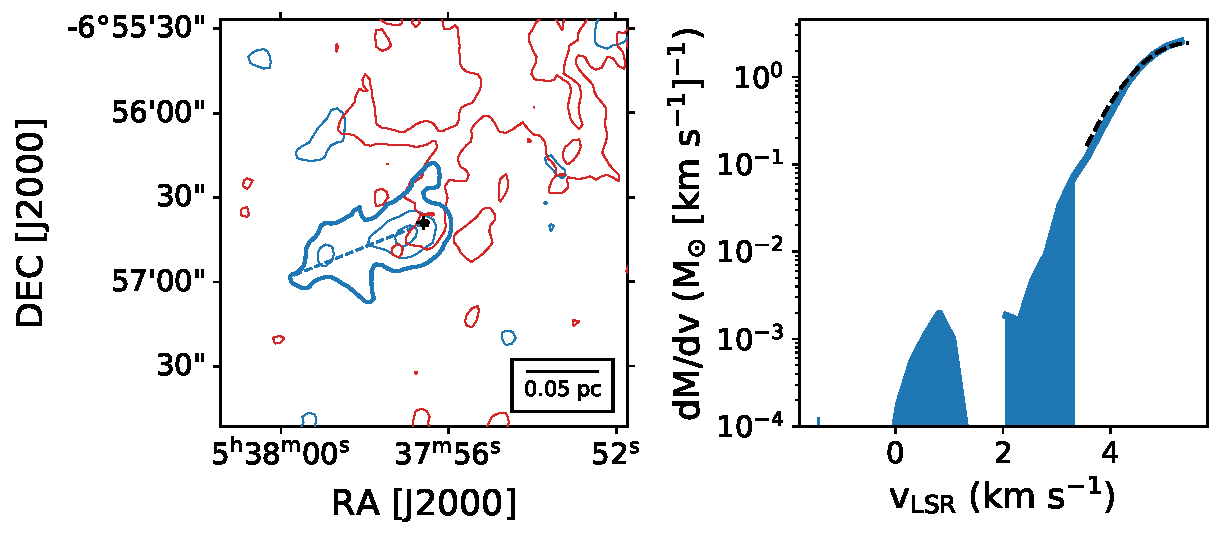
\includegraphics[width=\textwidth]{appendix_figures/hops157.pdf}

    \caption{HOPS 157 outflow. The left panel shows the outflow, position angle, nearby sources, and filaments.
    The velocity range of integration is given by v$_{\rm blue}$/v$_{\rm red}$ in Table~\ref{tab:outflows}
    and the contours go from $5$ to $50\sigma$ in steps of 5$\sigma$, where $\sigma$ is the RMS error in the integrated map. Symbols are the same as Figure~\ref{fig:stamp}.
    The right panel shows the mass spectrum with fit, where $\sigma$ is the RMS error in the integrated map. Symbols are the same as Figure~\ref{fig:dmdv}.}
    \end{figure*}
\begin{figure*}[p]
\centering
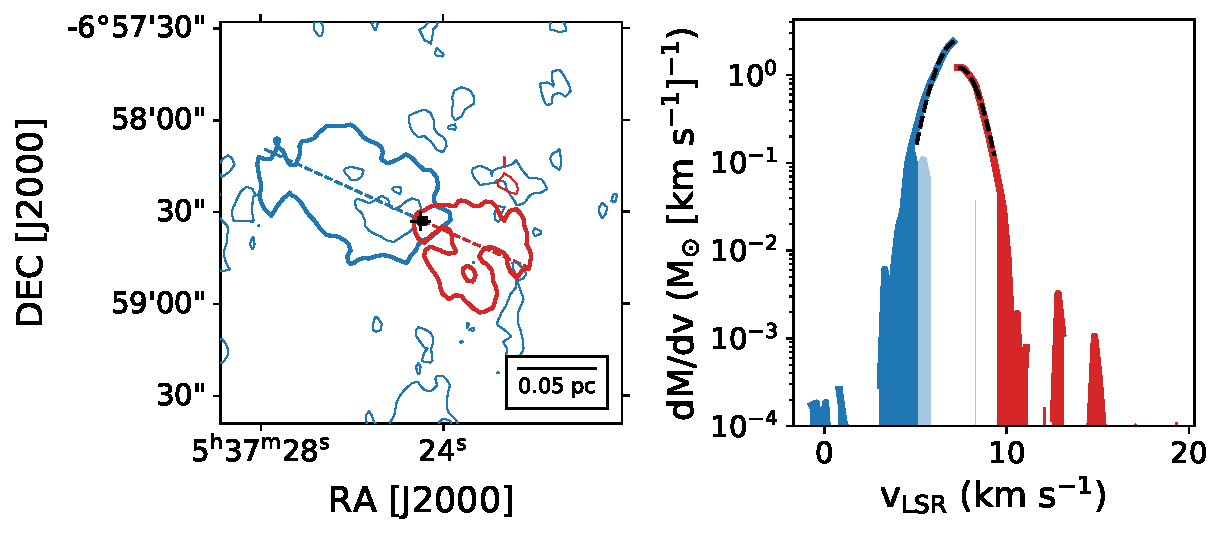
\includegraphics[width=\textwidth]{appendix_figures/hops158.pdf}

    \caption{HOPS 158 outflow. The left panel shows the outflow, position angle, nearby sources, and filaments.
    The velocity range of integration is given by v$_{\rm blue}$/v$_{\rm red}$ in Table~\ref{tab:outflows}
    and the contours go from $5$ to $50\sigma$ in steps of 5$\sigma$, where $\sigma$ is the RMS error in the integrated map. Symbols are the same as Figure~\ref{fig:stamp}.
    The right panel shows the mass spectrum with fit, where $\sigma$ is the RMS error in the integrated map. Symbols are the same as Figure~\ref{fig:dmdv}.}
    \end{figure*}
\begin{figure*}[p]
\centering
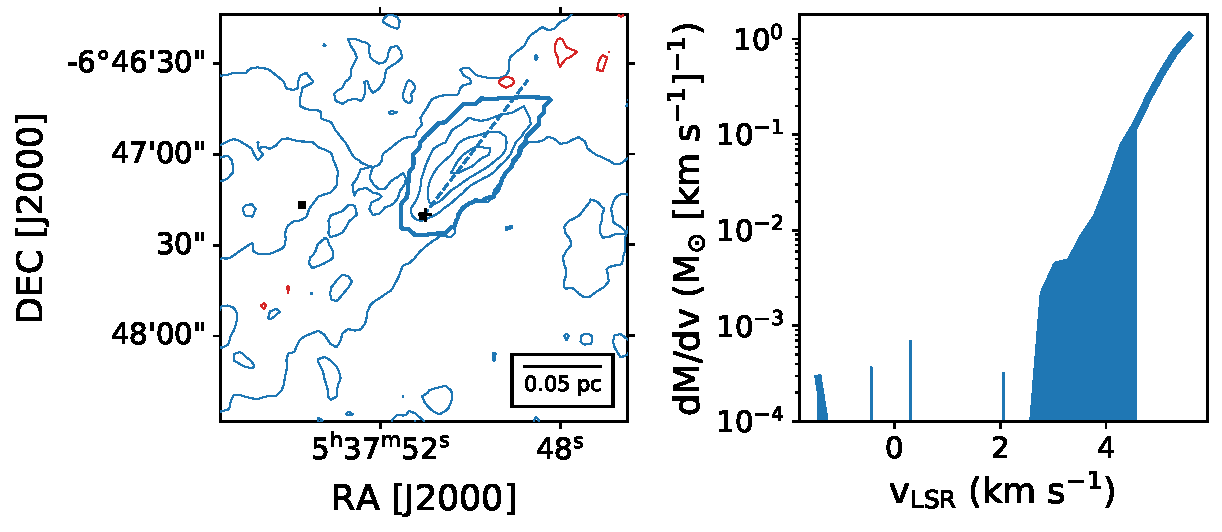
\includegraphics[width=\textwidth]{appendix_figures/hops160.pdf}

    \caption{HOPS 160 outflow. The left panel shows the outflow, position angle, nearby sources, and filaments.
    The velocity range of integration is given by v$_{\rm blue}$/v$_{\rm red}$ in Table~\ref{tab:outflows}
    and the contours go from $5$ to $50\sigma$ in steps of 5$\sigma$, where $\sigma$ is the RMS error in the integrated map. Symbols are the same as Figure~\ref{fig:stamp}.
    The right panel shows the mass spectrum with fit, where $\sigma$ is the RMS error in the integrated map. Symbols are the same as Figure~\ref{fig:dmdv}.}
    \end{figure*}
\begin{figure*}[p]
\centering
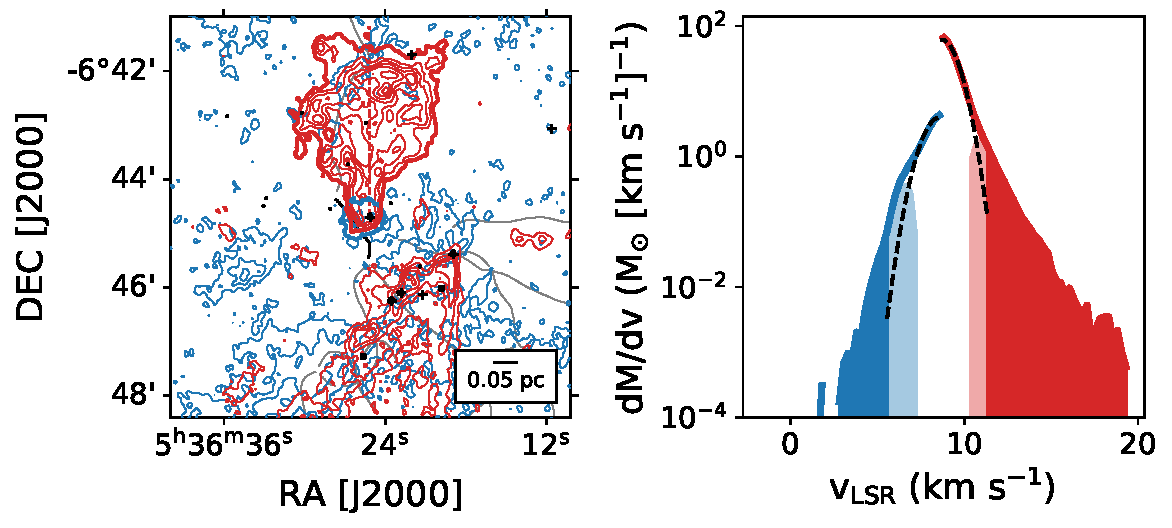
\includegraphics[width=\textwidth]{appendix_figures/hops166.pdf}

    \caption{HOPS 166 outflow. The left panel shows the outflow, position angle, nearby sources, and filaments.
    The velocity range of integration is given by v$_{\rm blue}$/v$_{\rm red}$ in Table~\ref{tab:outflows}
    and the contours go from $5$ to $50\sigma$ in steps of 5$\sigma$, where $\sigma$ is the RMS error in the integrated map. Symbols are the same as Figure~\ref{fig:stamp}.
    The right panel shows the mass spectrum with fit, where $\sigma$ is the RMS error in the integrated map. Symbols are the same as Figure~\ref{fig:dmdv}.}
    \end{figure*}
\begin{figure*}[p]
\centering
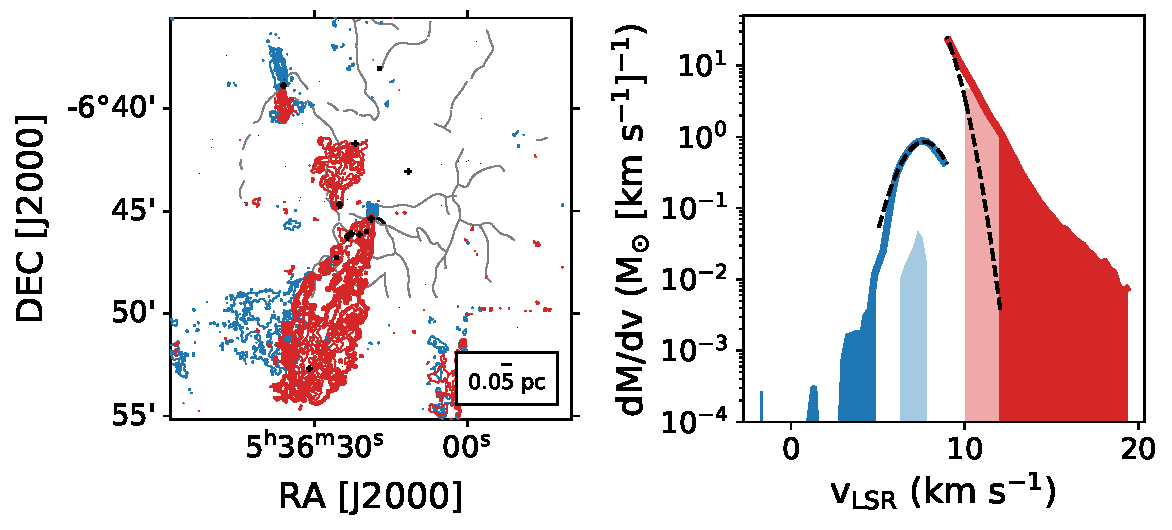
\includegraphics[width=\textwidth]{appendix_figures/hops168.pdf}

    \caption{HOPS 168 outflow. The left panel shows the outflow, position angle, nearby sources, and filaments.
    The velocity range of integration is given by v$_{\rm blue}$/v$_{\rm red}$ in Table~\ref{tab:outflows}
    and the contours go from $5$ to $50\sigma$ in steps of 5$\sigma$, where $\sigma$ is the RMS error in the integrated map. Symbols are the same as Figure~\ref{fig:stamp}.
    The right panel shows the mass spectrum with fit, where $\sigma$ is the RMS error in the integrated map. Symbols are the same as Figure~\ref{fig:dmdv}.}
    \end{figure*}
\begin{figure*}[p]
\centering
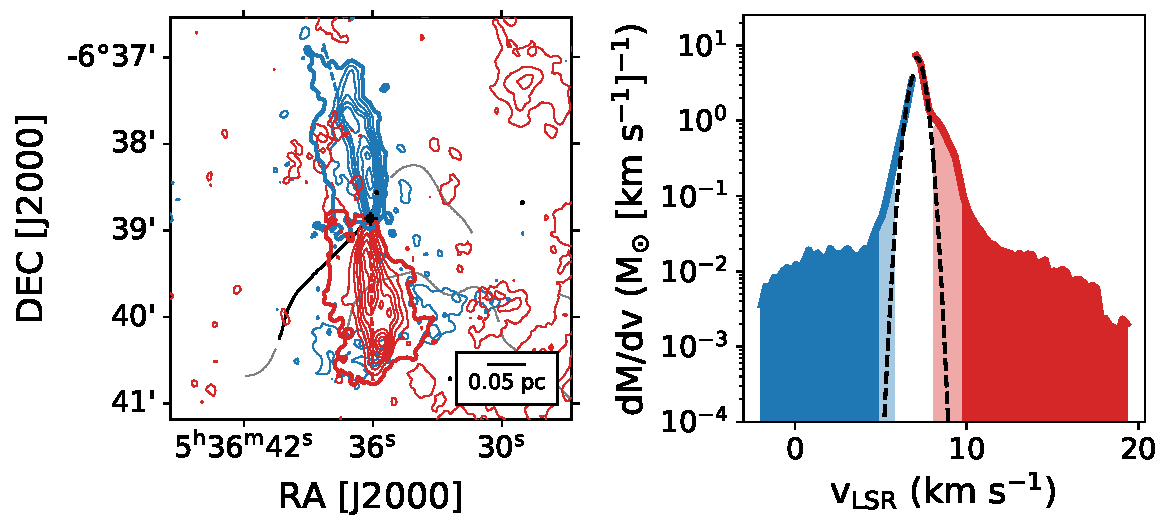
\includegraphics[width=\textwidth]{appendix_figures/hops169.pdf}

    \caption{HOPS 169 outflow. The left panel shows the outflow, position angle, nearby sources, and filaments.
    The velocity range of integration is given by v$_{\rm blue}$/v$_{\rm red}$ in Table~\ref{tab:outflows}
    and the contours go from $5$ to $50\sigma$ in steps of 5$\sigma$, where $\sigma$ is the RMS error in the integrated map. Symbols are the same as Figure~\ref{fig:stamp}.
    The right panel shows the mass spectrum with fit, where $\sigma$ is the RMS error in the integrated map. Symbols are the same as Figure~\ref{fig:dmdv}.}
    \end{figure*}
\begin{figure*}[p]
\centering
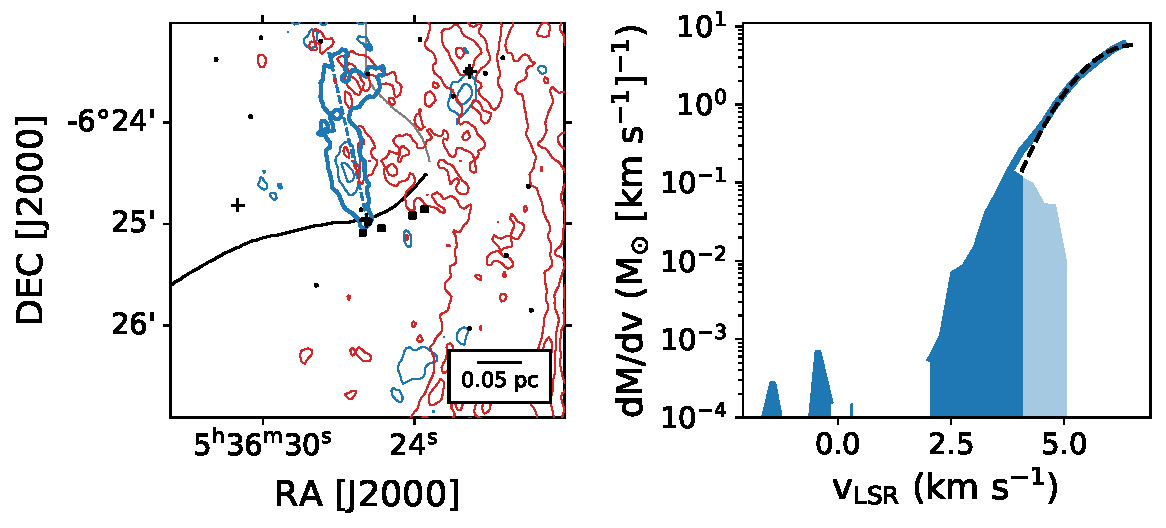
\includegraphics[width=\textwidth]{appendix_figures/hops174.pdf}

    \caption{HOPS 174 outflow. The left panel shows the outflow, position angle, nearby sources, and filaments.
    The velocity range of integration is given by v$_{\rm blue}$/v$_{\rm red}$ in Table~\ref{tab:outflows}
    and the contours go from $5$ to $50\sigma$ in steps of 5$\sigma$, where $\sigma$ is the RMS error in the integrated map. Symbols are the same as Figure~\ref{fig:stamp}.
    The right panel shows the mass spectrum with fit, where $\sigma$ is the RMS error in the integrated map. Symbols are the same as Figure~\ref{fig:dmdv}.}
    \end{figure*}
\begin{figure*}[p]
\centering
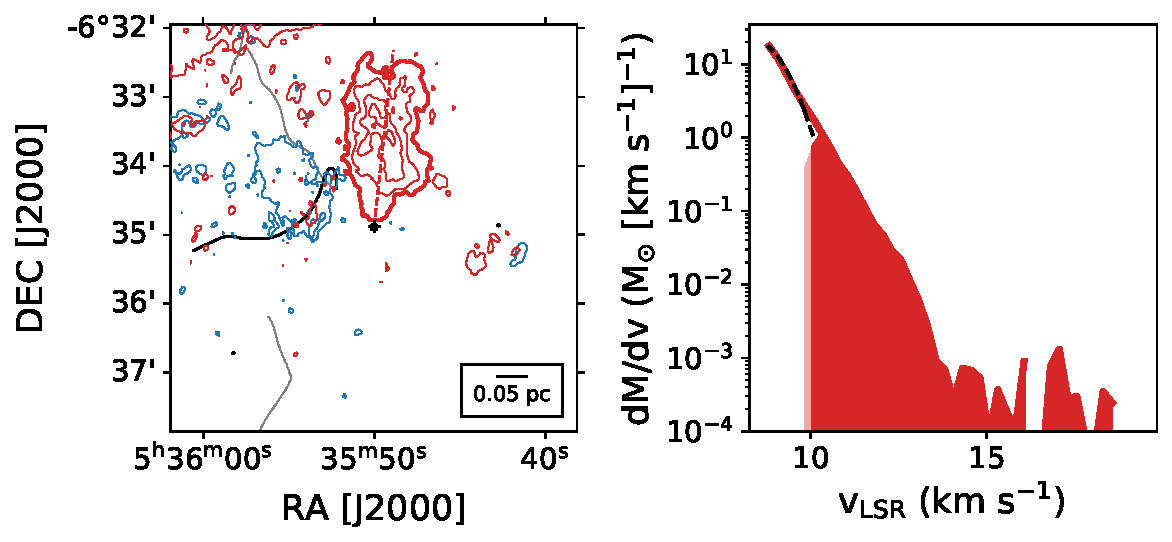
\includegraphics[width=\textwidth]{appendix_figures/hops177.pdf}

    \caption{HOPS 177 outflow. The left panel shows the outflow, position angle, nearby sources, and filaments.
    The velocity range of integration is given by v$_{\rm blue}$/v$_{\rm red}$ in Table~\ref{tab:outflows}
    and the contours go from $5$ to $50\sigma$ in steps of 5$\sigma$, where $\sigma$ is the RMS error in the integrated map. Symbols are the same as Figure~\ref{fig:stamp}.
    The right panel shows the mass spectrum with fit, where $\sigma$ is the RMS error in the integrated map. Symbols are the same as Figure~\ref{fig:dmdv}.}
    \end{figure*}
\begin{figure*}[p]
\centering
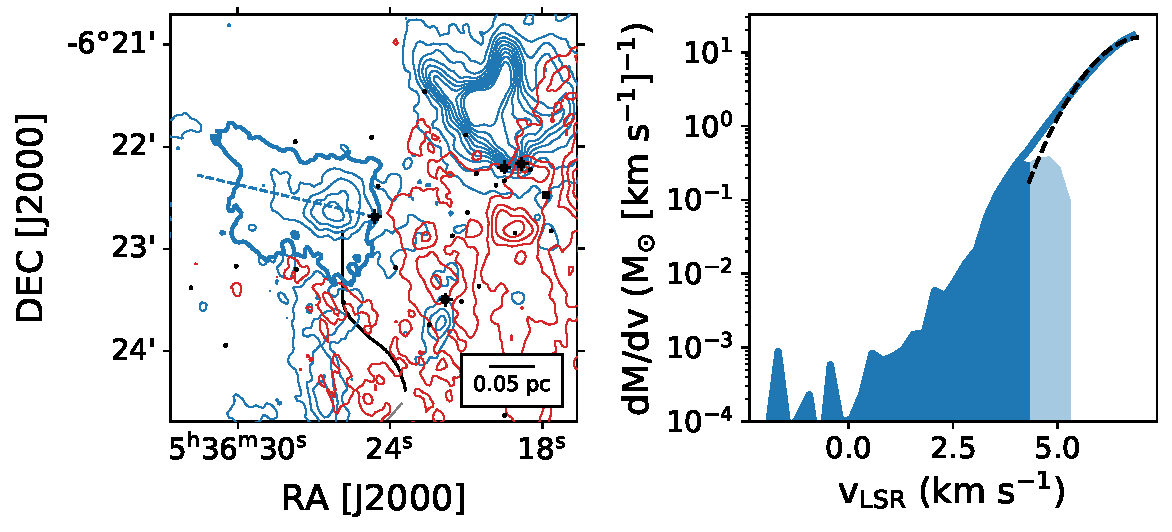
\includegraphics[width=\textwidth]{appendix_figures/hops178.pdf}

    \caption{HOPS 178 outflow. The left panel shows the outflow, position angle, nearby sources, and filaments.
    The velocity range of integration is given by v$_{\rm blue}$/v$_{\rm red}$ in Table~\ref{tab:outflows}
    and the contours go from $5$ to $50\sigma$ in steps of 5$\sigma$, where $\sigma$ is the RMS error in the integrated map. Symbols are the same as Figure~\ref{fig:stamp}.
    The right panel shows the mass spectrum with fit, where $\sigma$ is the RMS error in the integrated map. Symbols are the same as Figure~\ref{fig:dmdv}.}
    \end{figure*}
\begin{figure*}[p]
\centering
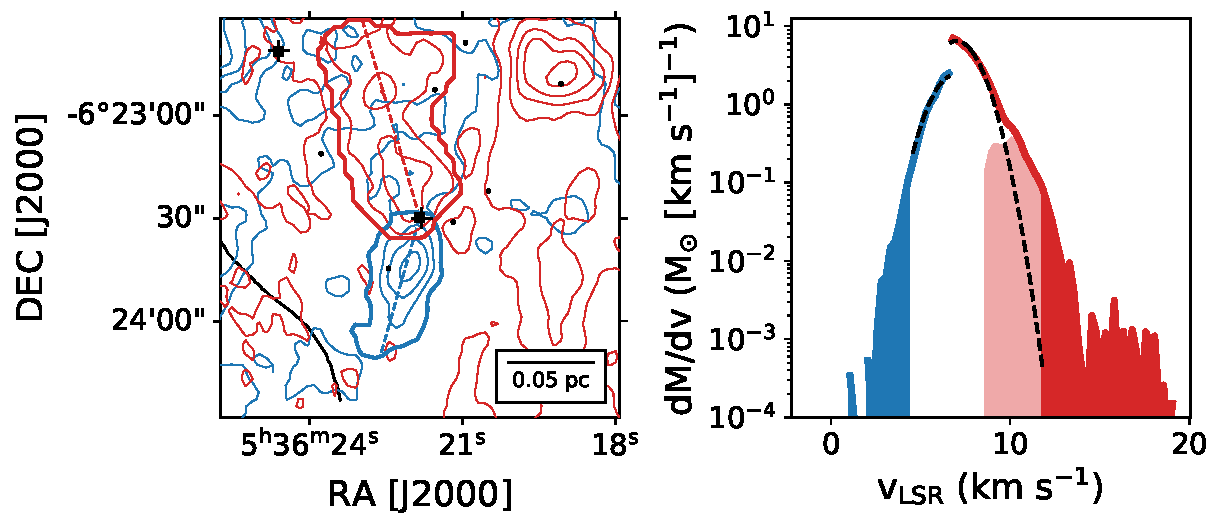
\includegraphics[width=\textwidth]{appendix_figures/hops179.pdf}

    \caption{HOPS 179 outflow. The left panel shows the outflow, position angle, nearby sources, and filaments.
    The velocity range of integration is given by v$_{\rm blue}$/v$_{\rm red}$ in Table~\ref{tab:outflows}
    and the contours go from $5$ to $50\sigma$ in steps of 5$\sigma$, where $\sigma$ is the RMS error in the integrated map. Symbols are the same as Figure~\ref{fig:stamp}.
    The right panel shows the mass spectrum with fit, where $\sigma$ is the RMS error in the integrated map. Symbols are the same as Figure~\ref{fig:dmdv}.}
    \end{figure*}
\begin{figure*}[p]
\centering
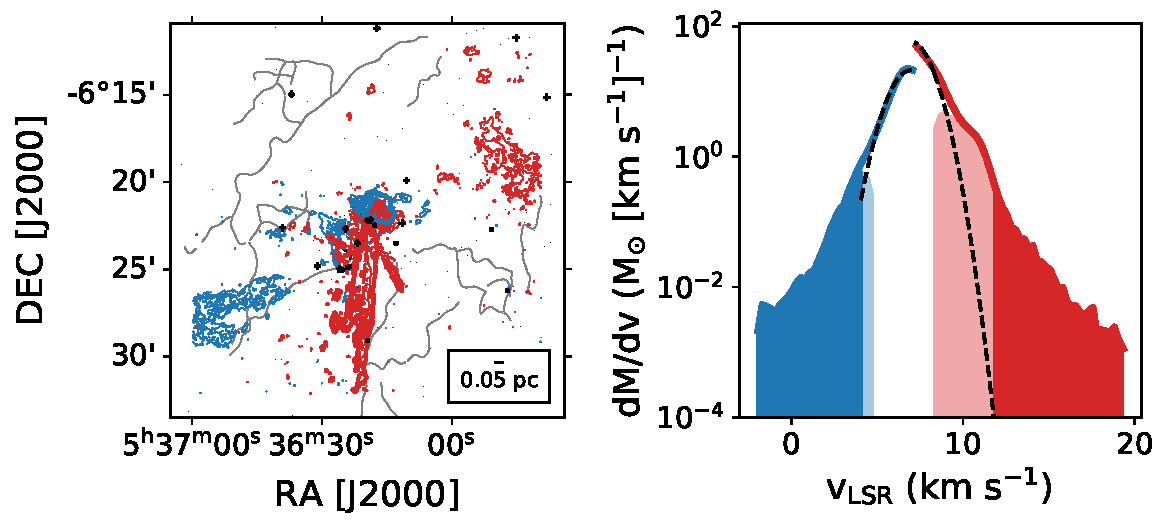
\includegraphics[width=\textwidth]{appendix_figures/hops181.pdf}

    \caption{HOPS 181 outflow. The left panel shows the outflow, position angle, nearby sources, and filaments.
    The velocity range of integration is given by v$_{\rm blue}$/v$_{\rm red}$ in Table~\ref{tab:outflows}
    and the contours go from $5$ to $50\sigma$ in steps of 5$\sigma$, where $\sigma$ is the RMS error in the integrated map. Symbols are the same as Figure~\ref{fig:stamp}.
    The right panel shows the mass spectrum with fit, where $\sigma$ is the RMS error in the integrated map. Symbols are the same as Figure~\ref{fig:dmdv}.}
    \end{figure*}
\begin{figure*}[p]
\centering
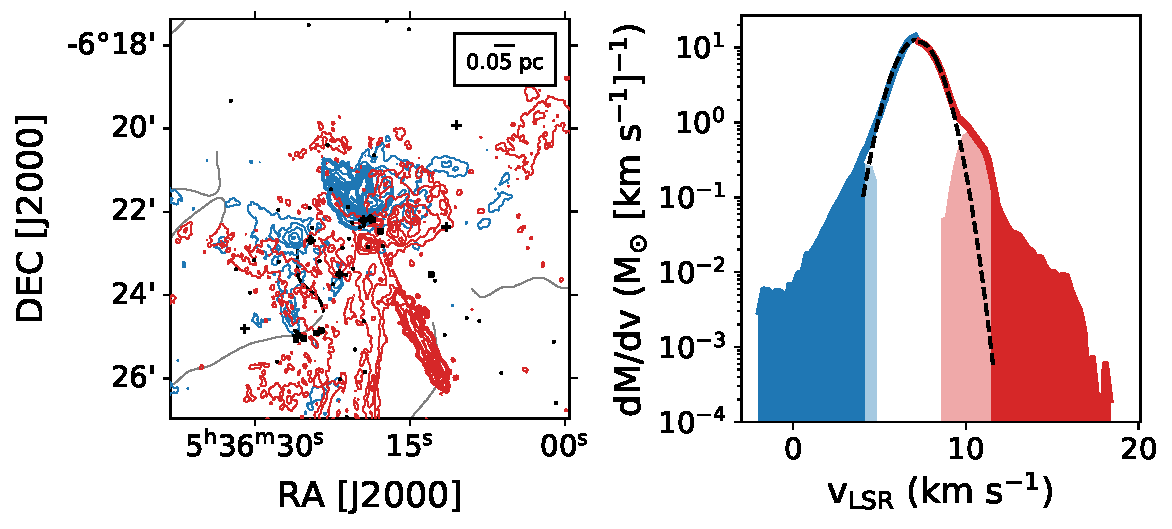
\includegraphics[width=\textwidth]{appendix_figures/hops182.pdf}

    \caption{HOPS 182 outflow. The left panel shows the outflow, position angle, nearby sources, and filaments.
    The velocity range of integration is given by v$_{\rm blue}$/v$_{\rm red}$ in Table~\ref{tab:outflows}
    and the contours go from $5$ to $50\sigma$ in steps of 5$\sigma$, where $\sigma$ is the RMS error in the integrated map. Symbols are the same as Figure~\ref{fig:stamp}.
    The right panel shows the mass spectrum with fit, where $\sigma$ is the RMS error in the integrated map. Symbols are the same as Figure~\ref{fig:dmdv}.}
    \end{figure*}
\begin{figure*}[p]
\centering
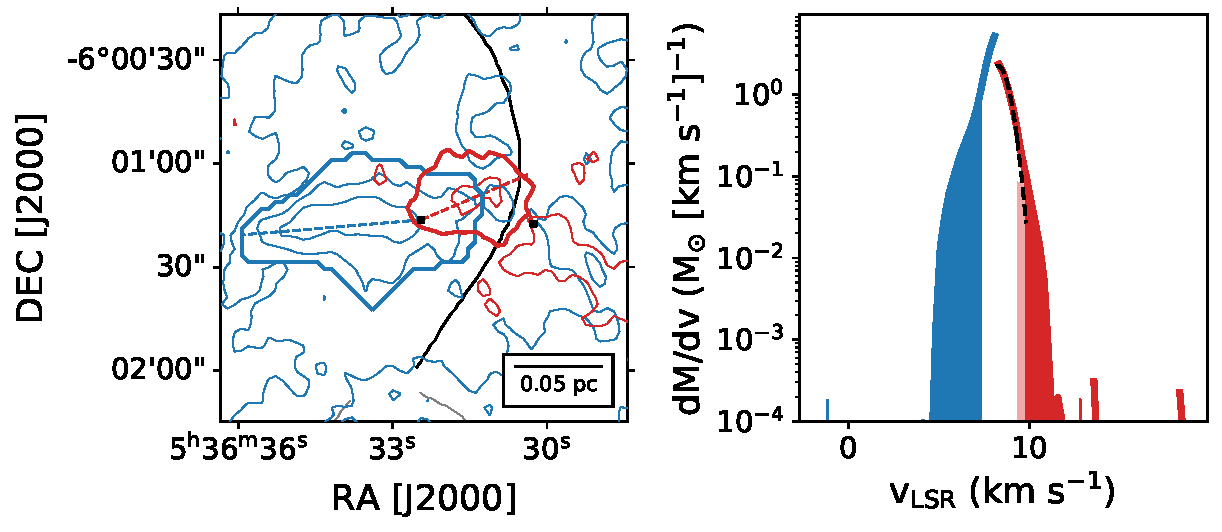
\includegraphics[width=\textwidth]{appendix_figures/hops192.pdf}

    \caption{HOPS 192 outflow. The left panel shows the outflow, position angle, nearby sources, and filaments.
    The velocity range of integration is given by v$_{\rm blue}$/v$_{\rm red}$ in Table~\ref{tab:outflows}
    and the contours go from $5$ to $50\sigma$ in steps of 5$\sigma$, where $\sigma$ is the RMS error in the integrated map. Symbols are the same as Figure~\ref{fig:stamp}.
    The right panel shows the mass spectrum with fit, where $\sigma$ is the RMS error in the integrated map. Symbols are the same as Figure~\ref{fig:dmdv}.}
    \end{figure*}
\begin{figure*}[p]
\centering
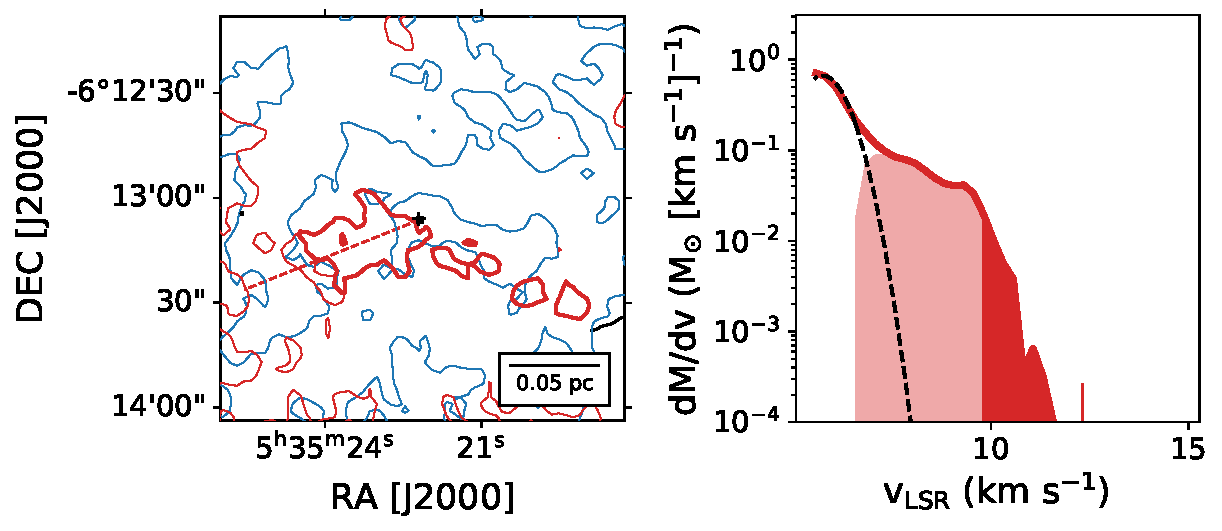
\includegraphics[width=\textwidth]{appendix_figures/hops198.pdf}

    \caption{HOPS 198 outflow. The left panel shows the outflow, position angle, nearby sources, and filaments.
    The velocity range of integration is given by v$_{\rm blue}$/v$_{\rm red}$ in Table~\ref{tab:outflows}
    and the contours go from $5$ to $50\sigma$ in steps of 5$\sigma$, where $\sigma$ is the RMS error in the integrated map. Symbols are the same as Figure~\ref{fig:stamp}.
    The right panel shows the mass spectrum with fit, where $\sigma$ is the RMS error in the integrated map. Symbols are the same as Figure~\ref{fig:dmdv}.}
    \end{figure*}
\begin{figure*}[p]
\centering
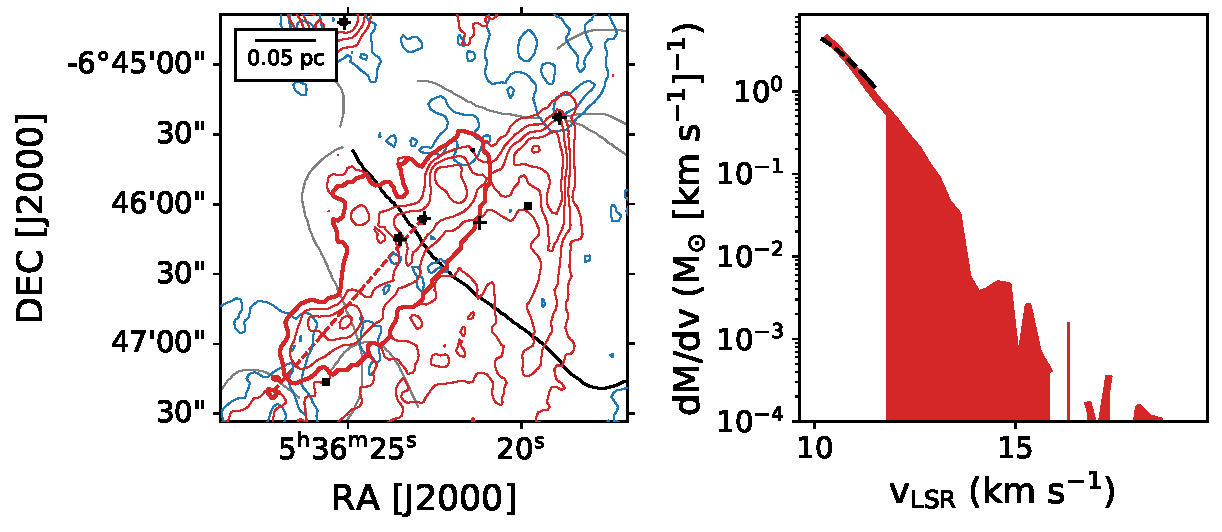
\includegraphics[width=\textwidth]{appendix_figures/hops203.pdf}

    \caption{HOPS 203 outflow. The left panel shows the outflow, position angle, nearby sources, and filaments.
    The velocity range of integration is given by v$_{\rm blue}$/v$_{\rm red}$ in Table~\ref{tab:outflows}
    and the contours go from $5$ to $50\sigma$ in steps of 5$\sigma$, where $\sigma$ is the RMS error in the integrated map. Symbols are the same as Figure~\ref{fig:stamp}.
    The right panel shows the mass spectrum with fit, where $\sigma$ is the RMS error in the integrated map. Symbols are the same as Figure~\ref{fig:dmdv}.}
    \end{figure*}
\begin{figure*}[p]
\centering
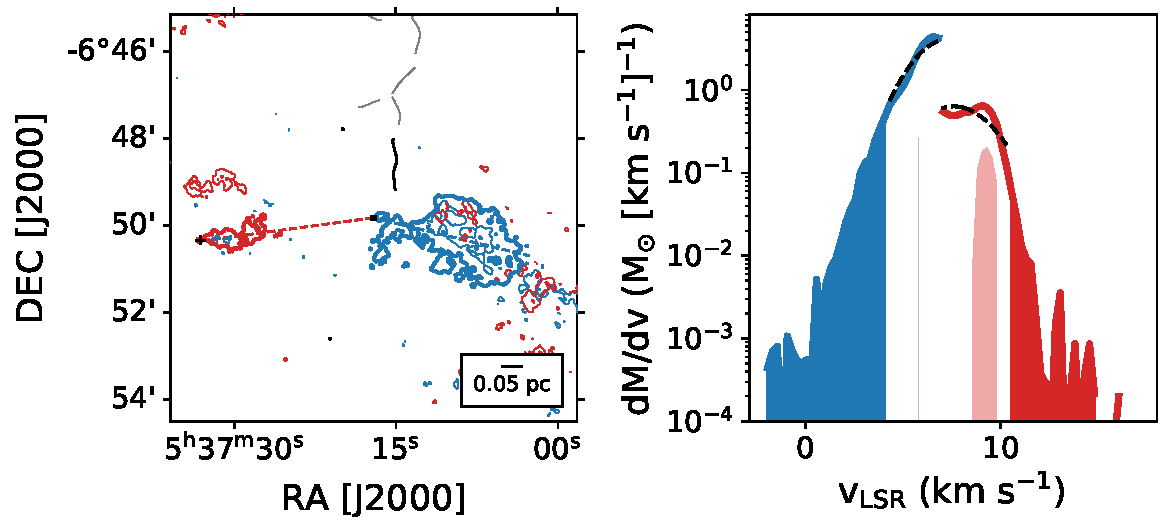
\includegraphics[width=\textwidth]{appendix_figures/hops355.pdf}

    \caption{HOPS 355 outflow. The left panel shows the outflow, position angle, nearby sources, and filaments.
    The velocity range of integration is given by v$_{\rm blue}$/v$_{\rm red}$ in Table~\ref{tab:outflows}
    and the contours go from $5$ to $50\sigma$ in steps of 5$\sigma$, where $\sigma$ is the RMS error in the integrated map. Symbols are the same as Figure~\ref{fig:stamp}.
    The right panel shows the mass spectrum with fit, where $\sigma$ is the RMS error in the integrated map. Symbols are the same as Figure~\ref{fig:dmdv}.}
    \end{figure*}
\begin{figure*}[p]
\centering
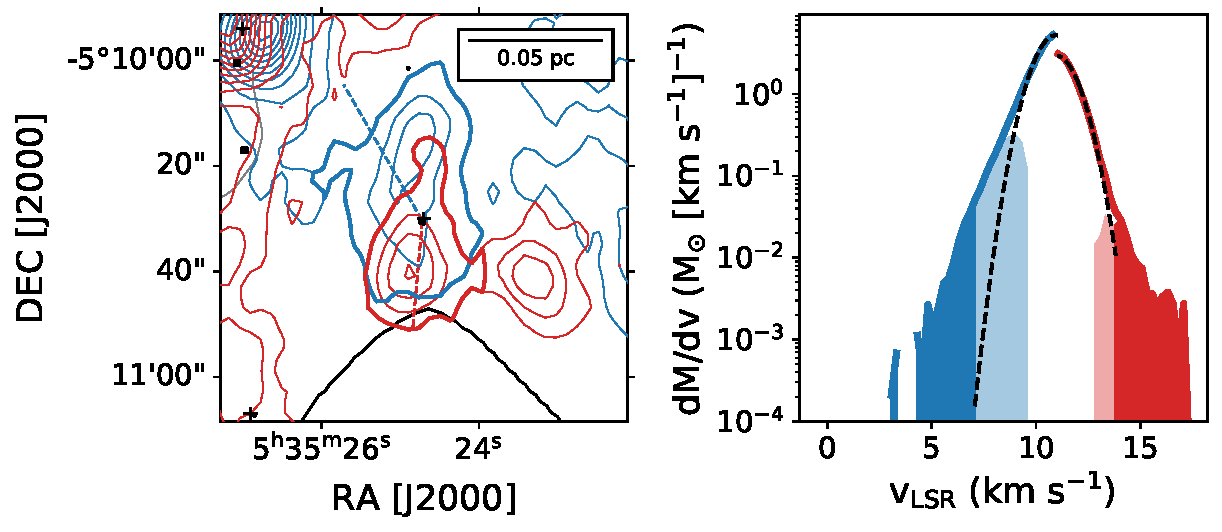
\includegraphics[width=\textwidth]{appendix_figures/hops368.pdf}

    \caption{HOPS 368 outflow. The left panel shows the outflow, position angle, nearby sources, and filaments.
    The velocity range of integration is given by v$_{\rm blue}$/v$_{\rm red}$ in Table~\ref{tab:outflows}
    and the contours go from $5$ to $50\sigma$ in steps of 5$\sigma$, where $\sigma$ is the RMS error in the integrated map. Symbols are the same as Figure~\ref{fig:stamp}.
    The right panel shows the mass spectrum with fit, where $\sigma$ is the RMS error in the integrated map. Symbols are the same as Figure~\ref{fig:dmdv}.}
    \end{figure*}
\begin{figure*}[p]
\centering
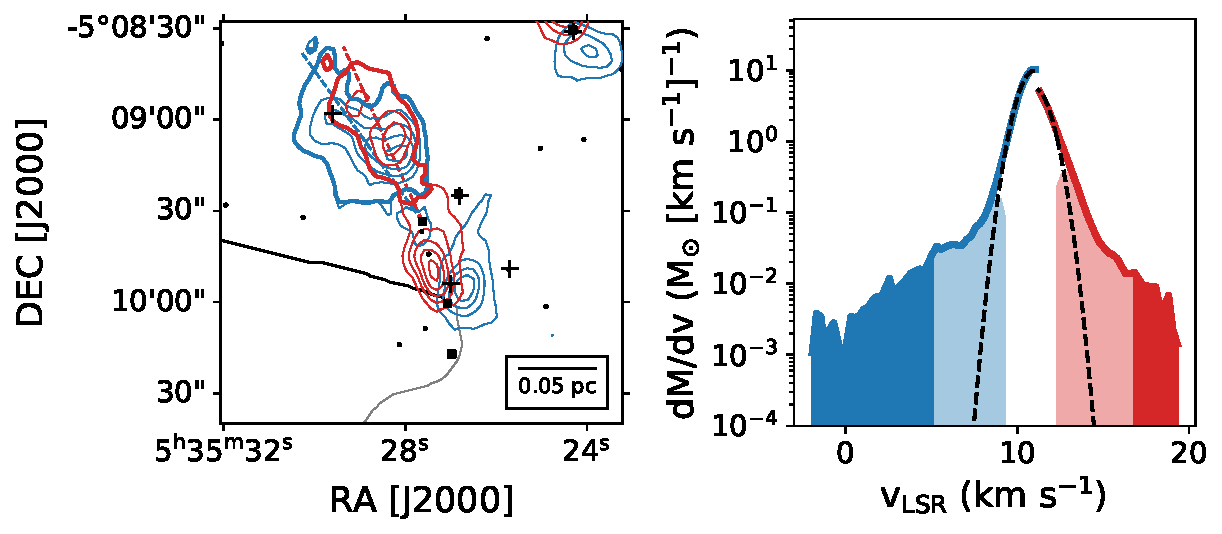
\includegraphics[width=\textwidth]{appendix_figures/hops370.pdf}

    \caption{HOPS 370 outflow. The left panel shows the outflow, position angle, nearby sources, and filaments.
    The velocity range of integration is given by v$_{\rm blue}$/v$_{\rm red}$ in Table~\ref{tab:outflows}
    and the contours go from $5$ to $50\sigma$ in steps of 5$\sigma$, where $\sigma$ is the RMS error in the integrated map. Symbols are the same as Figure~\ref{fig:stamp}.
    The right panel shows the mass spectrum with fit, where $\sigma$ is the RMS error in the integrated map. Symbols are the same as Figure~\ref{fig:dmdv}.}
    \end{figure*}
\begin{figure*}[p]
\centering
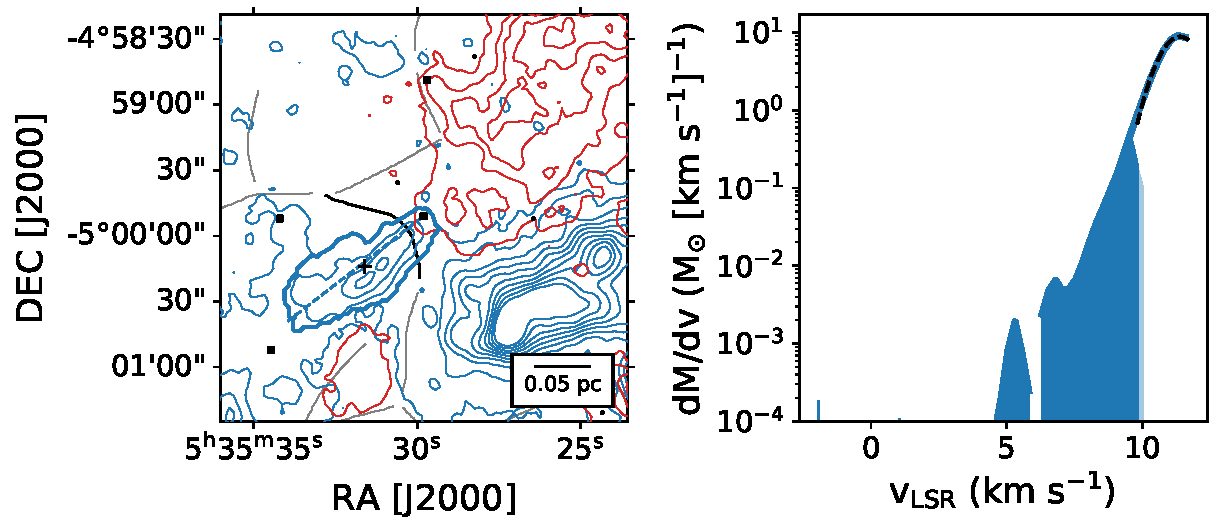
\includegraphics[width=\textwidth]{appendix_figures/hops383.pdf}

    \caption{HOPS 383 outflow. The left panel shows the outflow, position angle, nearby sources, and filaments.
    The velocity range of integration is given by v$_{\rm blue}$/v$_{\rm red}$ in Table~\ref{tab:outflows}
    and the contours go from $5$ to $50\sigma$ in steps of 5$\sigma$, where $\sigma$ is the RMS error in the integrated map. Symbols are the same as Figure~\ref{fig:stamp}.
    The right panel shows the mass spectrum with fit, where $\sigma$ is the RMS error in the integrated map. Symbols are the same as Figure~\ref{fig:dmdv}.}
    \end{figure*}
